\section{Experiments}
\label{sec-experiments-main}
\begin{figure}[ht]
\begin{tabular}{cc} 
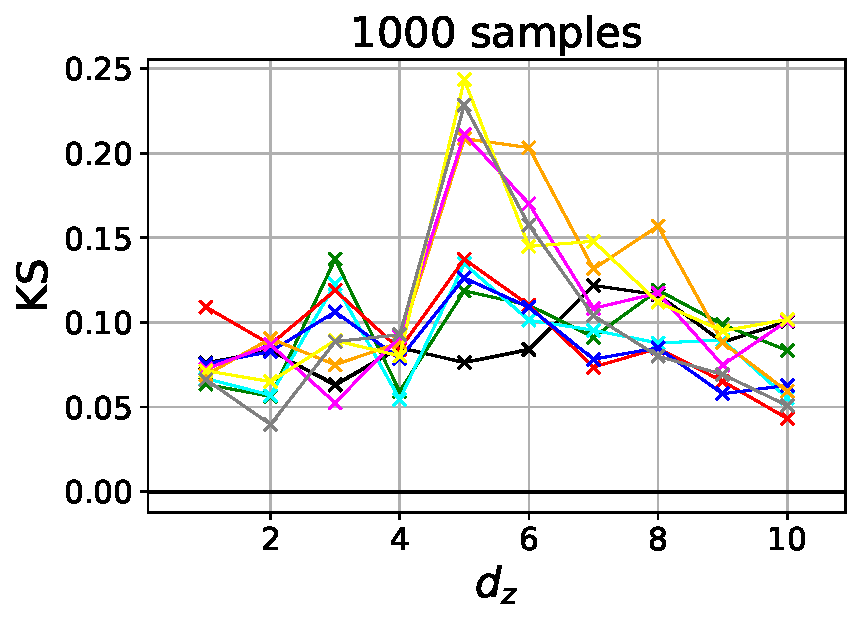
\includegraphics[height=3.7cm]{sections/appendix/independence_testing_kernel/figures_J_p/fig_ours_J_p_ks.pdf}& 
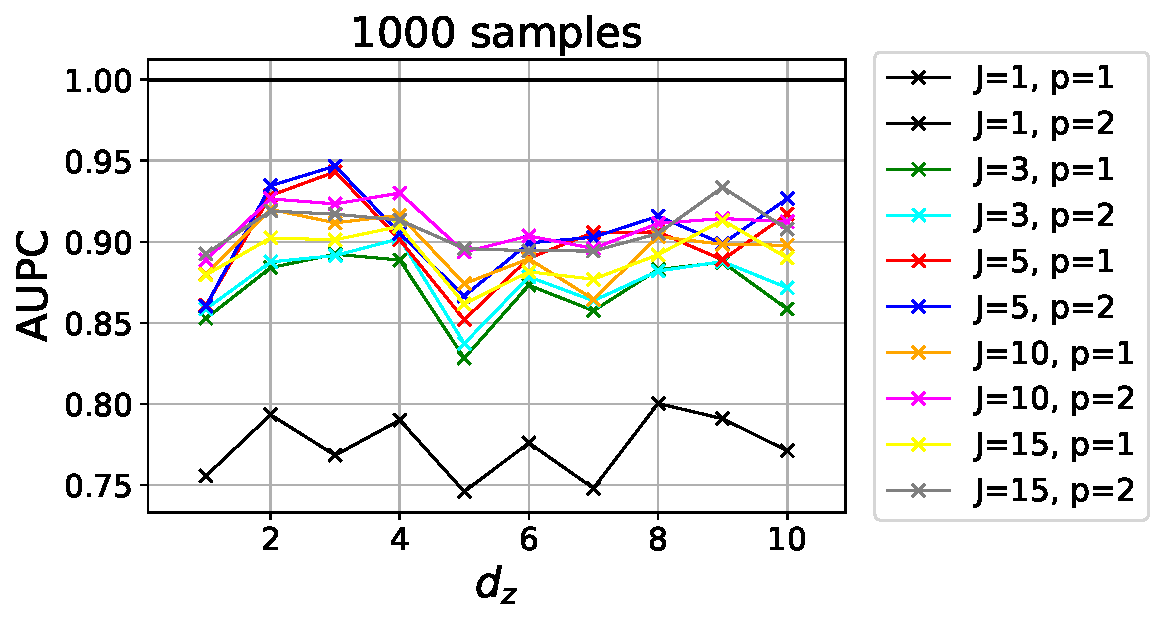
\includegraphics[height=3.7cm]{sections/appendix/independence_testing_kernel/figures_J_p/fig_ours_J_p_aupc.pdf}
\end{tabular}
\caption{Comparison of the KS statistic (\emph{left}) and the AUPC (\emph{right}) of our test statistic $\widetilde{\text{NCI}}_{n,r,p}$ when the data is generated respectively from the models defined in~\eqref{exp-strobl-h0} and~\eqref{exp-strobl-h1} with Gaussian noises for multiple $p$ and $J$. For each problem, we draw $n=1000$ samples and repeat the experiment 100 times. We set $r=1000$ and report the results obtained when varying the dimension $d_z$ of each problem from 1 to 10. Observe that when $J=1$, for all $p\geq 1$ $\widetilde{\text{NCI}}_{n,r,1}=\widetilde{\text{NCI}}_{n,r,p}$, therefore there is only one  common black curve.
\label{fig-exp-param}}
\vspace{-0.4cm}
\end{figure}

\begin{figure}[ht]
\begin{tabular}{cc} 
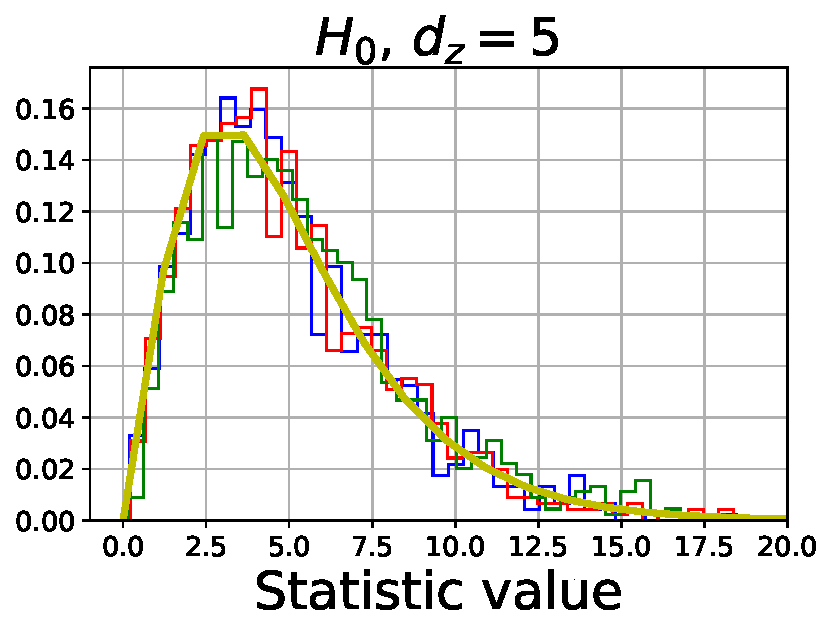
\includegraphics[width=0.24\textwidth]{sections/appendix/independence_testing_kernel/new_figures_oracle/oracle_h0_dim_5.pdf} 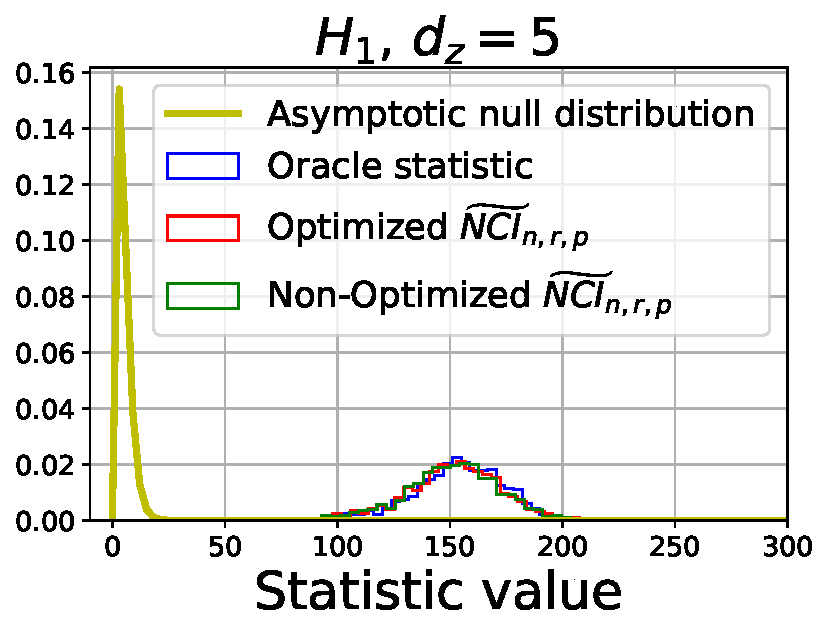
\includegraphics[width=0.24\textwidth]{sections/appendix/independence_testing_kernel/new_figures_oracle/oracle_h1_dim_5.pdf}  
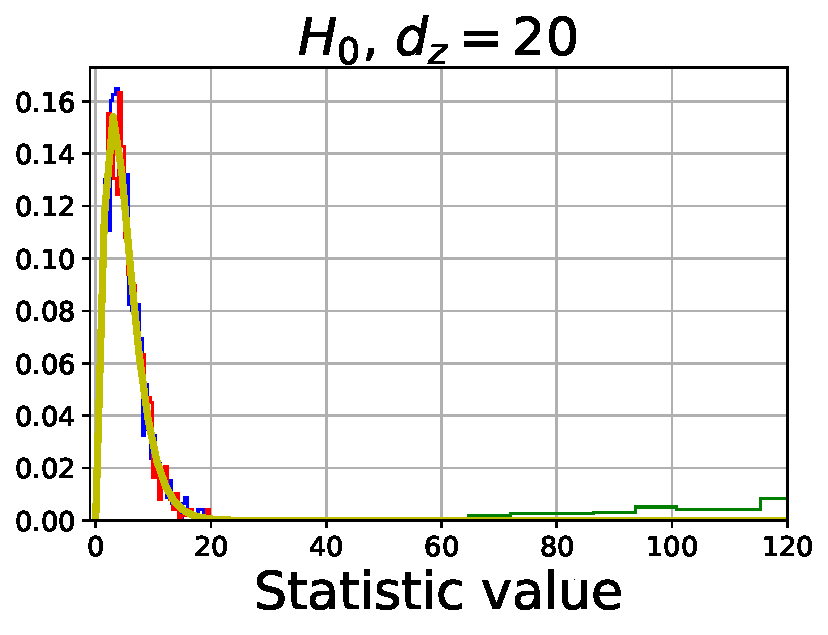
\includegraphics[width=0.24\textwidth]{sections/appendix/independence_testing_kernel/new_figures_oracle/oracle_h0_dim_20.pdf} 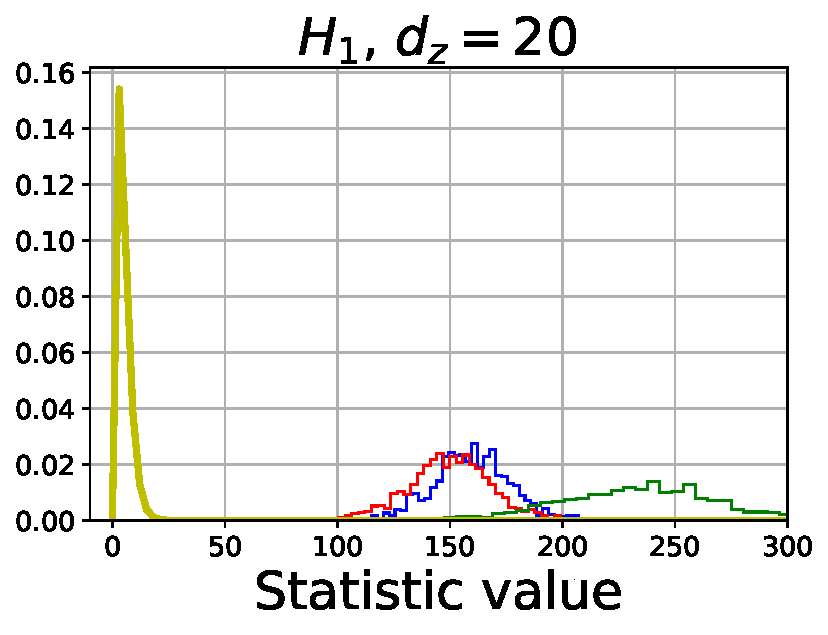
\includegraphics[width=0.24\textwidth]{sections/appendix/independence_testing_kernel/new_figures_oracle/oracle_h1_dim_20.pdf}
\end{tabular} 
\caption{Comparisons between the empirical distributions of the normalized version of the oracle statistic  $\widehat{\text{CI}}_{n,p}$ and the approximate normalized statistic $\widetilde{\text{NCI}}_{n,r,p}$, with the theoretical asymptotic null distribution when the data is generated either from the model defined in~\eqref{exp-illustration-h0} (\emph{left}) or the one defined in~\eqref{exp-illustration-h1} (\emph{right}). We set the dimension of $Z$ to be either $d_z=5$ (\emph{top row}) or $d_z=20$ (\emph{bottom row}). For each problem, we draw $n=1000$ samples and repeat the experiment 1000 times. In all the experiments, we set $J=5$ and $p=2$, thus the asymptotic null distribution follows a $\chi^2(5)$. Observe that both the oracle statistic and the approximated one recover the true asymptotic distribution under the null hypothesis. When $H_1$ holds, we can see that the two statistics manage to reject the null hypothesis. This figure also illustrates the empirical distribution of our approximate statistic when we do not optimize the hyperparameters involved in the RLS estimators: in this case we do not control the type-I error in the high dimensional setting.\label{fig-illustation-theory}}
\vspace{-0.4cm}
\end{figure}



% \begin{figure*}[tb]
% \begin{tabular}{cccc} 
% 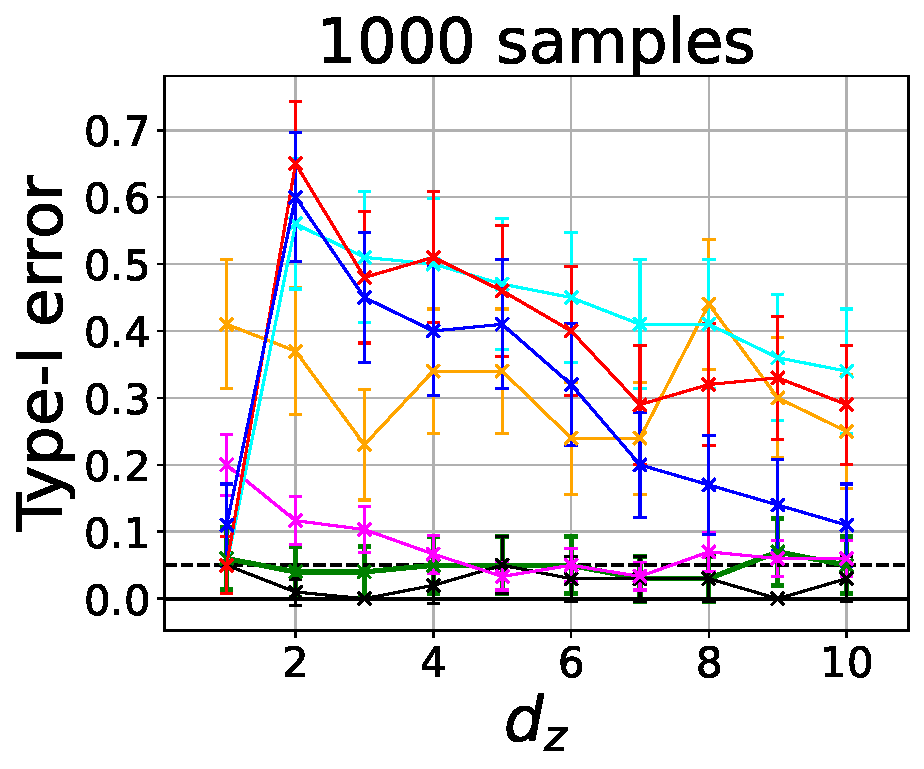
\includegraphics[height=3cm]{new_figures/nsamples_fixed_1000_li_dim_1_10_typeI.pdf}& 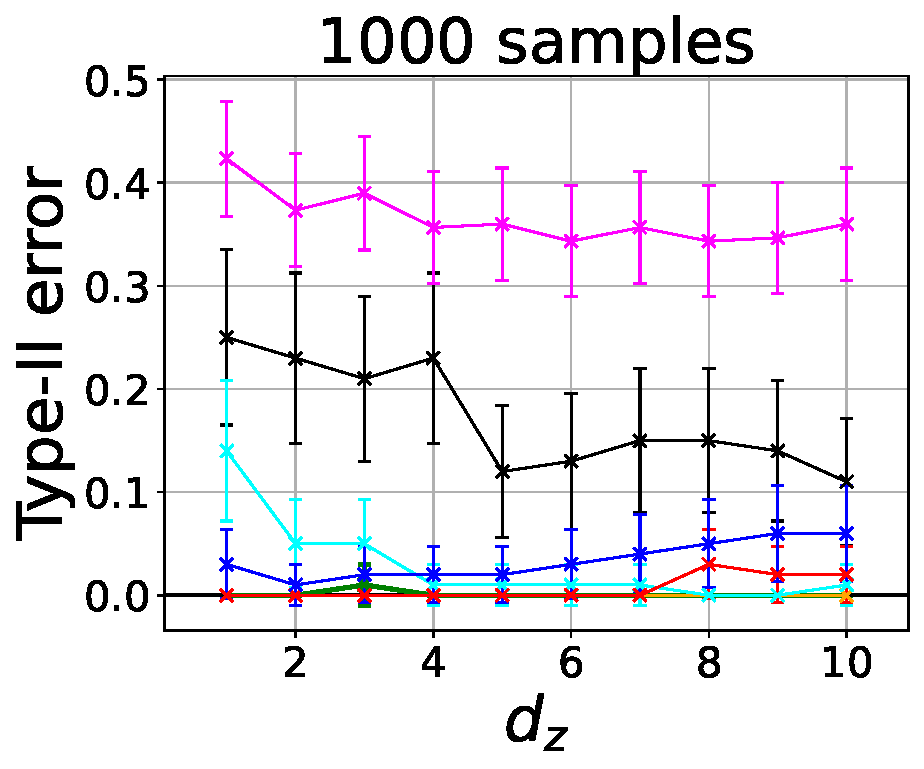
\includegraphics[height=3cm]{new_figures/nsamples_fixed_1000_li_dim_1_10_typeII.pdf} & 
% 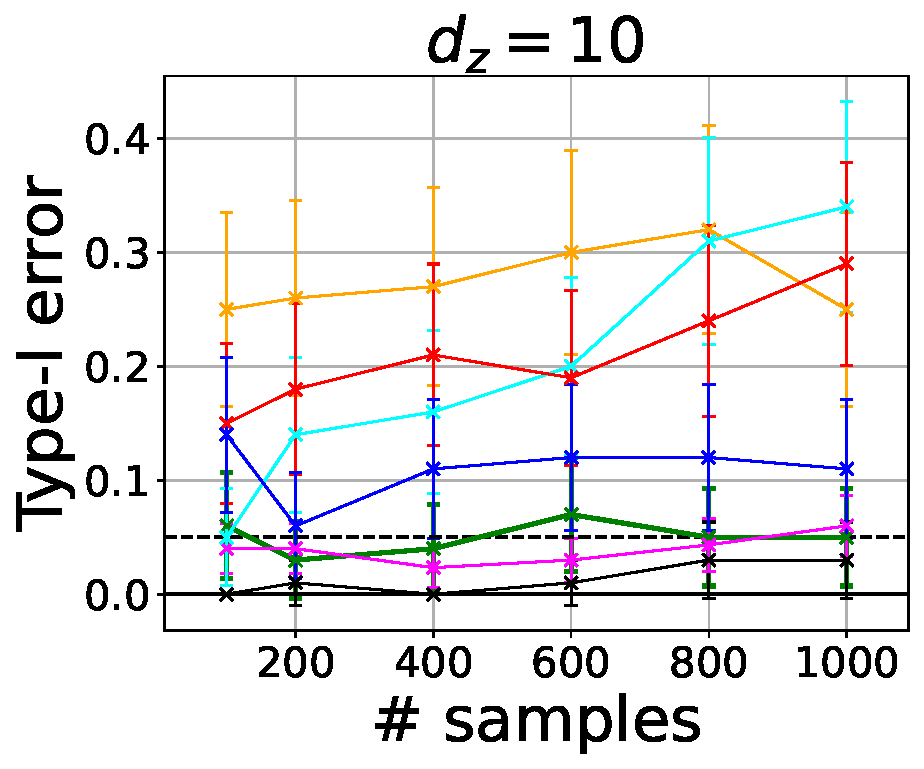
\includegraphics[height=3cm]{new_figures/dim_fixed_10_li_typeI.pdf}& 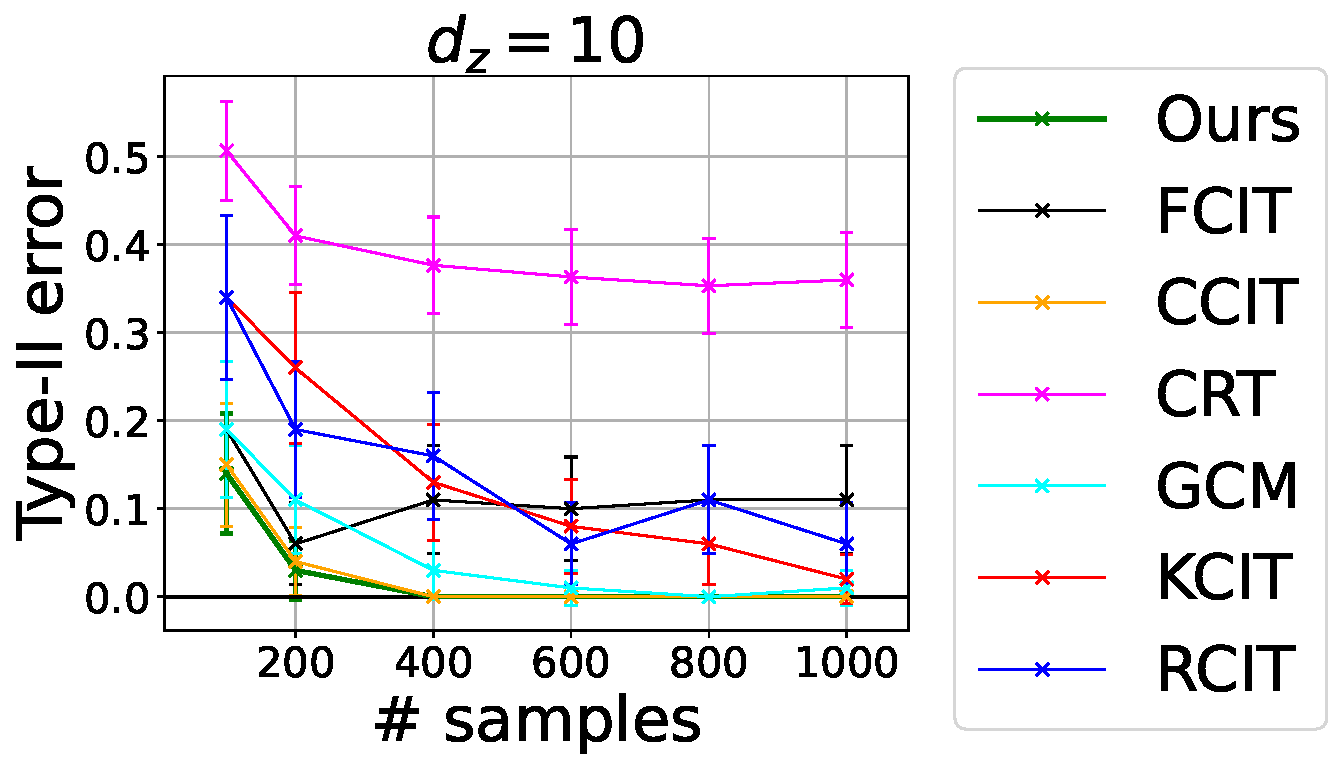
\includegraphics[height=3cm]{new_figures/dim_fixed_10_li_typeII.pdf} 
% \end{tabular}
% \caption{Comparison of the type-I error at level $\alpha=0.05$ (dashed line) and the type-II error (lower is better) of our test procedure with other SoTA tests on the two problems presented in~\eqref{li-exp-h0} and~\eqref{li-exp-h1}  with Gaussian noises. Each point in the figures is obtained by repeating the experiment for 100 independent trials. (\emph{Left, middle-left}): type-I and type-II errors obtained by each test when varying the dimension $d_z$ from 1 to 10; here, the number of samples $n$ is fixed and equals to $1000$. (\emph{Middle-right, right}): type-I and type-II errors obtained by each test when varying the number of samples $n$ from 100 to 1000; here, the dimension $d_z$ is fixed and equals to $10$. These experiments show that our method outperforms other tests as it manages to consistently control the type-I error and it is the most powerful. 
% \label{fig-exp-li}}
% \vspace{-0.3cm}
% \end{figure*}

% \begin{figure*}[ht]
% \begin{tabular}{cccc} 
% 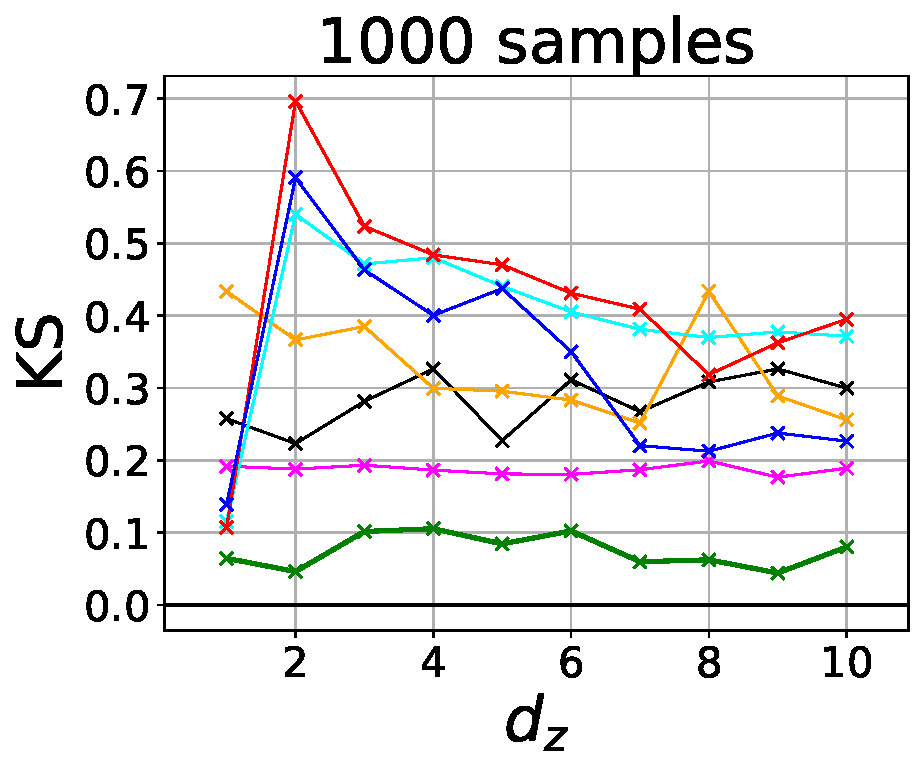
\includegraphics[height=2.3cm]{figures_supp_mat/nsamples_fixed_1000_li_dim_1_10_ks.pdf}& 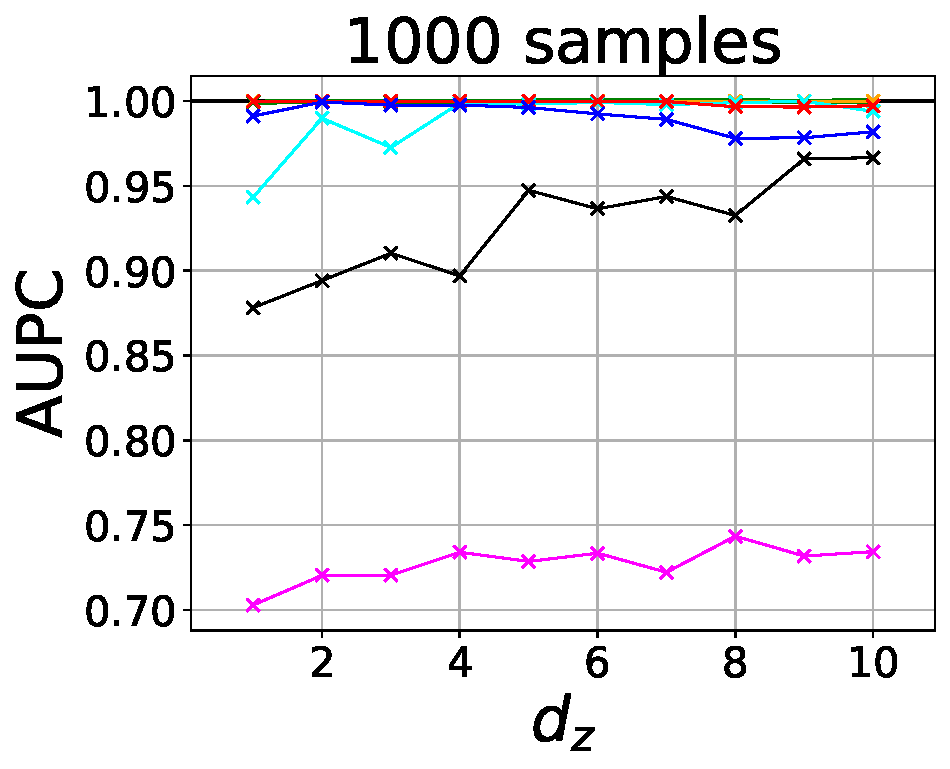
\includegraphics[height=2.3cm]{figures_supp_mat/nsamples_fixed_1000_li_dim_1_10_aupc.pdf} & 
% 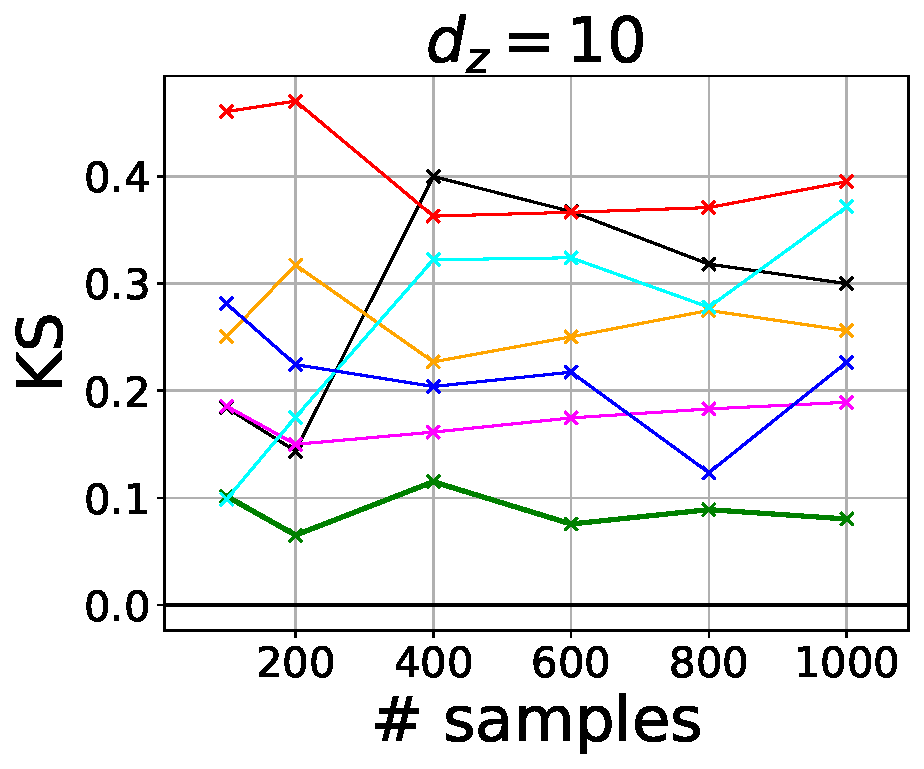
\includegraphics[height=2.3cm]{figures_supp_mat/dim_fixed_10_li_ks.pdf}& 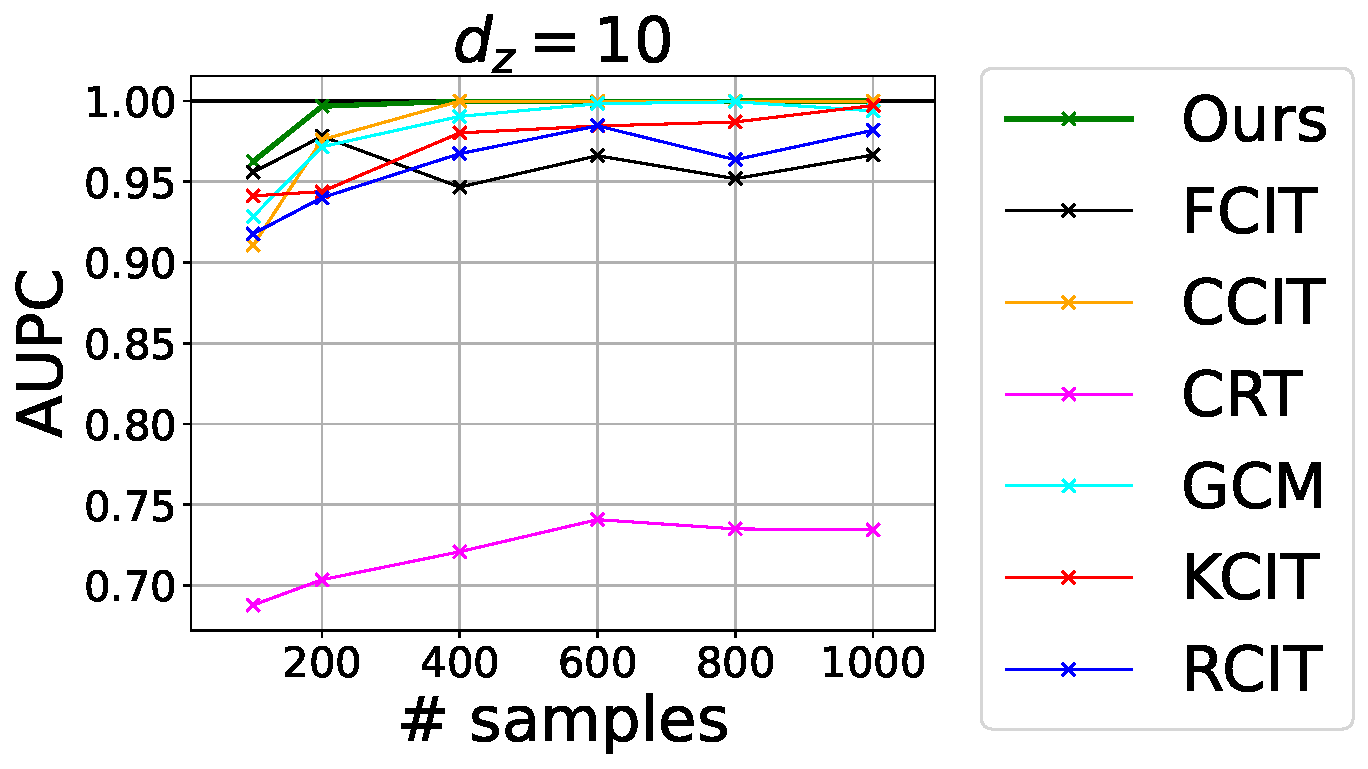
\includegraphics[height=2.3cm]{figures_supp_mat/dim_fixed_10_li_aupc.pdf}
% \end{tabular}
% \caption{Comparison of the KS statistic and the AUPC of our testing procedure with other SoTA tests on the two problems presented in Eq.~\eqref{li-exp-h0} and Eq.~\eqref{li-exp-h1} with Gaussian noises. Each point in the figures is obtained by repeating the experiment for 100 independent trials. (\emph{Left, middle-left}): the KS statistic and AUPC (respectively) obtained by each test when varying the dimension $d_z$ from 1 to 10; here, the number of samples $n$ is fixed and equals to $1000$. (\emph{Middle-right, right}): the KS and AUPC (respectively), obtained by each test when varying the number of samples $n$ from 100 to 1000; here, the dimension $d_z$ is fixed and equals to $10$.
% \label{fig-exp-li-ks}}
% \vspace{-0.3cm}
% \end{figure*}

\begin{figure*}[h]
\begin{tabular}{cccc} 
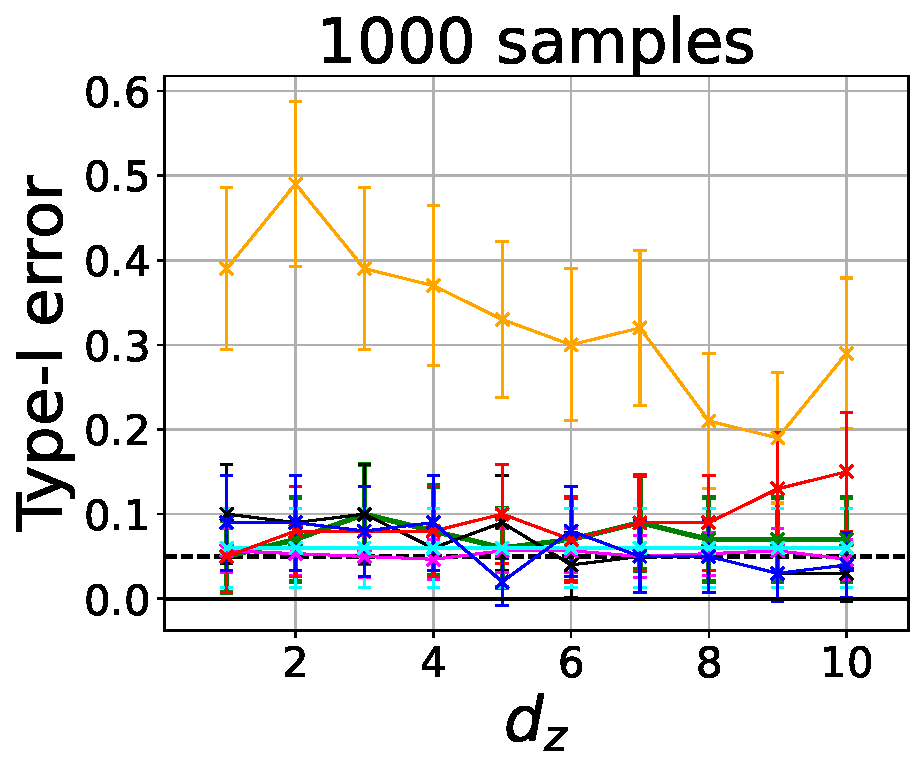
\includegraphics[height=2.3cm]{sections/appendix/independence_testing_kernel/figures_strobl_gaussian/nsamples_fixed_1000_strobl_dim_1_10_typeI.pdf}& 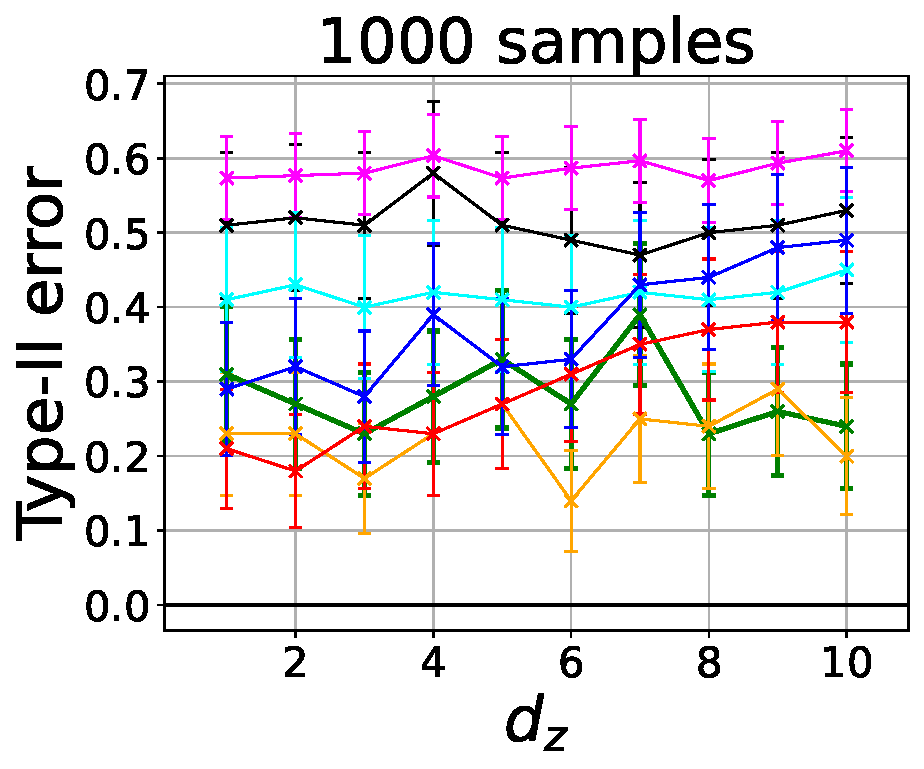
\includegraphics[height=2.3cm]{sections/appendix/independence_testing_kernel/figures_strobl_gaussian/nsamples_fixed_1000_strobl_dim_1_10_typeII.pdf} & 
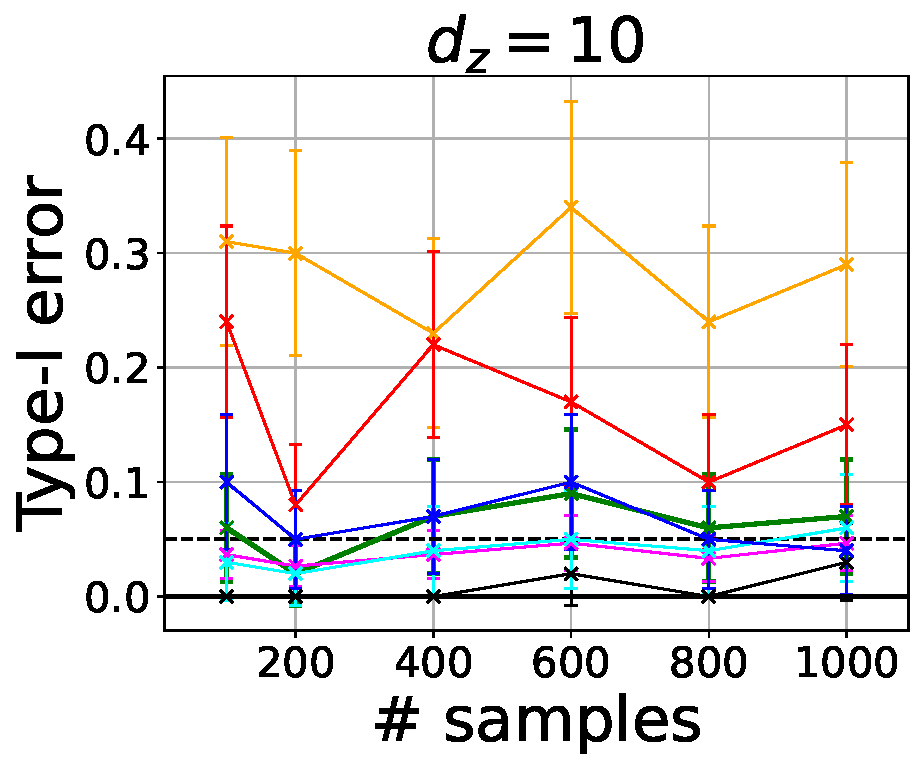
\includegraphics[height=2.3cm]{sections/appendix/independence_testing_kernel/figures_strobl_gaussian/dim_fixed_10_strobl_typeI.pdf}& 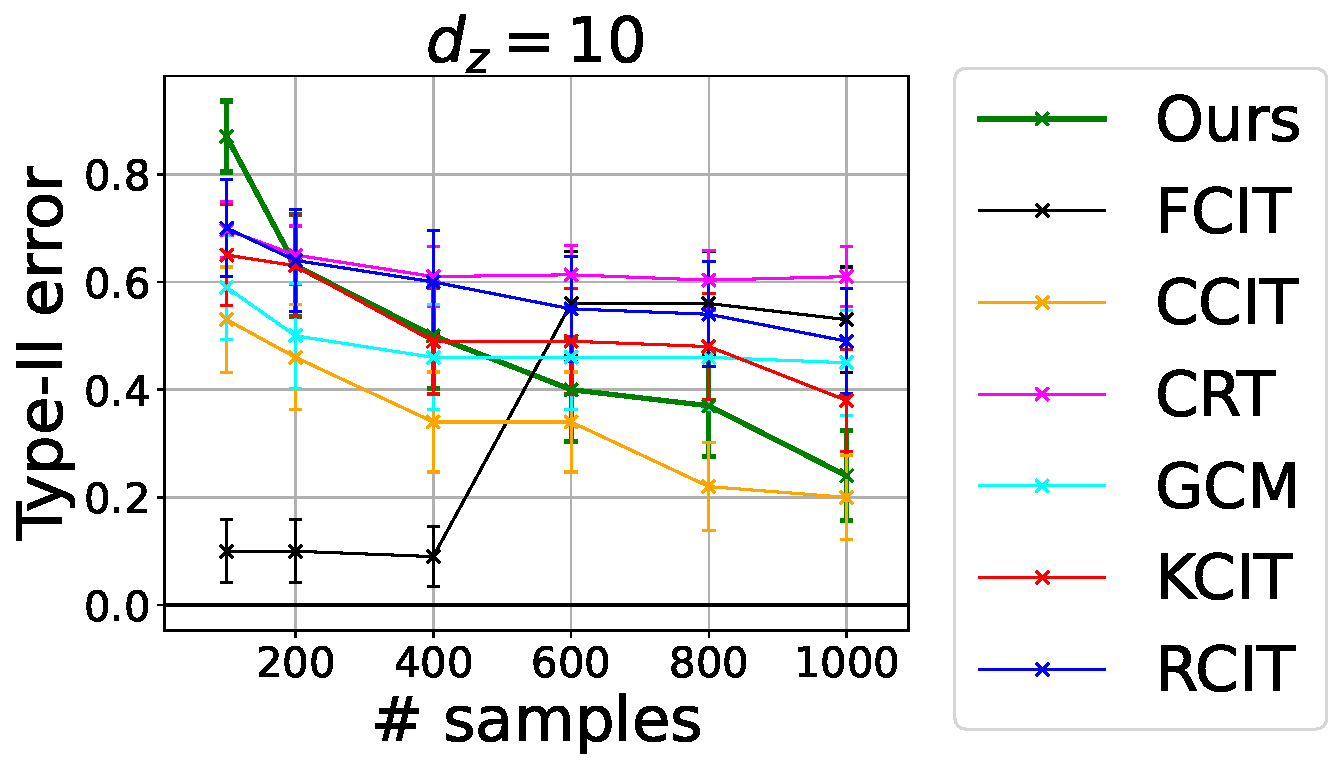
\includegraphics[height=2.3cm]{sections/appendix/independence_testing_kernel/figures_strobl_gaussian/dim_fixed_10_strobl_typeII.pdf}
\end{tabular}
\caption{Comparison of the type-I error at level $\alpha=0.05$ (dashed line) and the type-II error (lower is better) of our test procedure with other SoTA tests on the two problems presented in~\eqref{exp-strobl-h0} and~\eqref{exp-strobl-h1}  with Gaussian noises. Each point in the figures is obtained by repeating the experiment for 100 independent trials. (\emph{Left, middle-left}): type-I and type-II errors obtained by each test when varying the dimension $d_z$ from 1 to 10; here, the number of samples $n$ is fixed and equals to $1000$. (\emph{Middle-right, right}): type-I and type-II errors obtained by each test when varying the number of samples $n$ from 100 to 1000; here, the dimension $d_z$ is fixed and equals to $10$. 
\label{fig-exp-strobl-type}}
\vspace{-0.3cm}
\end{figure*}




The goal of this section is three fold: (i) to investigate the effects of the parameters $J$ and $p$ on the performances of our method, (ii) to validate our theoretical results depicted in Propositions~\ref{prop:oracle-law} and \ref{prop:norm-law}, and (iii) to compare our method with those proposed in the literature. In more detail, we first compare the performance of our method, both in terms of both power and type-I error, by varying the hyperparameters $J$ and $p$. We show that our method is robust to the choice of $p$, and also show that the power increases as $J$ increases. Then, we explore synthetic toy problems where one can derive an explicit formulation of the conditional means involved in our test statistic. In these cases, we can compute our proposed oracle statistic $\widehat{\text{CI}}_{n,p}$ and its normalized version, allowing us to show that under the null hypothesis we recover the theoretical asymptotic null distribution obtained in Proposition~\ref{prop:oracle-law}. We also reach to similar conclusions regarding our approximate normalized test statistic, $\widetilde{\text{NCI}}_{n,r,p}$. In addition, in this experiment, we investigate the effect of the proposed optimization procedure for choosing the hyperparameters involved in the RLS estimators of $\widetilde{\text{NCI}}_{n,r,p}$, and show its benefits. Finally, we demonstrate on several synthetic experiments that our proposed testing procedure outperforms state-of-the-art (SoTA) methods both in terms of statistical power and type-I error, even in the high dimensional setting. 




\textbf{Benchmarks.} We consider 6 synthetic data sets and compare the power and type-I error of our test $\widetilde{\text{NCI}}_{n,r,p}$ to the following 6 existing CI methods: \textbf{KCIT}~\citep{zhang2012kernel}, \textbf{RCIT}~\citep{strobl2019approximate}, \textbf{CCIT}~\citep{sen2017modelpowered}, \textbf{CRT}~\citep{candes2018panning} using correlation statistic from \citep{BellotS19}, \textbf{FCIT}~\citep{chalupka2018fast} and \textbf{GCM}~\citep{gcm2020}. Software packages of all the above tests are freely available online and each experiment was run on a single CPU. 





\textbf{Evaluation.} To evaluate the performance of the tests, we consider four metrics. Under $H_0$, we report either the Kolmogorov-Smirnov (KS) test statistic between the distribution of p-values returned by the tests and the uniform distribution on $[0,1]$, or the type-I errors at level $\alpha=0.05$. Note that a valid conditional independence test should control the type-I error rate at any level $\alpha$. Here, a test that generates a p-value that follows the uniform distribution over $[0,1]$ will achieve this requirement. The latter property of the p-values translates to a small KS statistic value. Under $H_1$, we compute either the area under the power curve (AUPC) of the empirical cumulative density function of the p-values returned by the tests, or the resulting type-II error. A conditional test has higher power when its AUPC is closer to one. Alternatively, the smaller the type-II error is, the more powerful the test is.

% \begin{figure*}[htb]
% \begin{tabular}{cccc} 
% 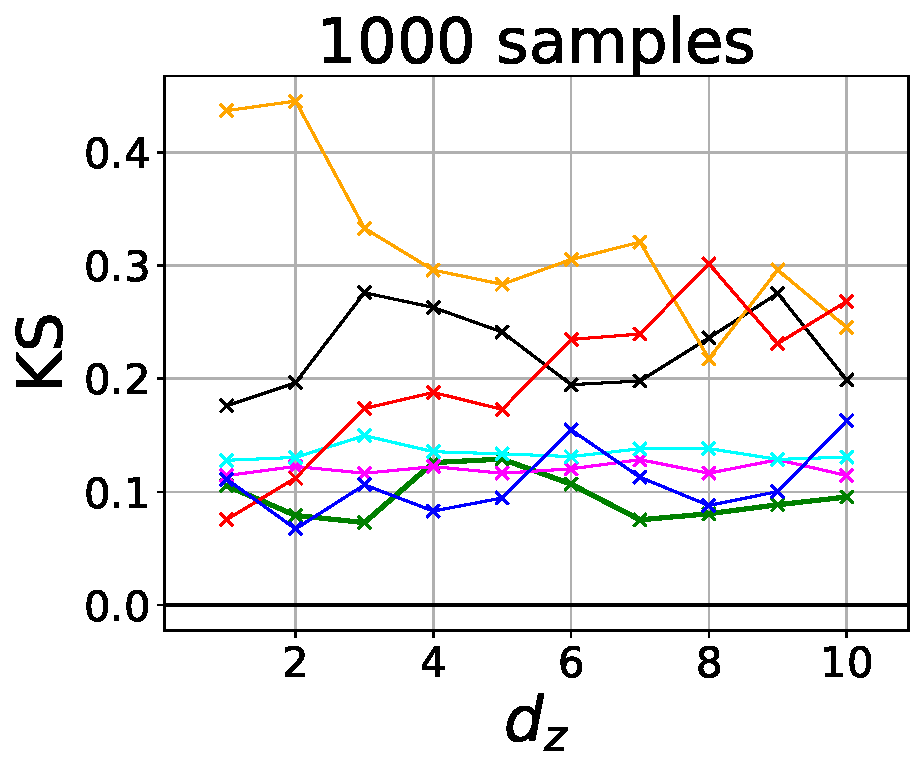
\includegraphics[height=2.3cm]{new_figures_lap/nsamples_fixed_1000_strobl_dim_1_10_ks.pdf}& 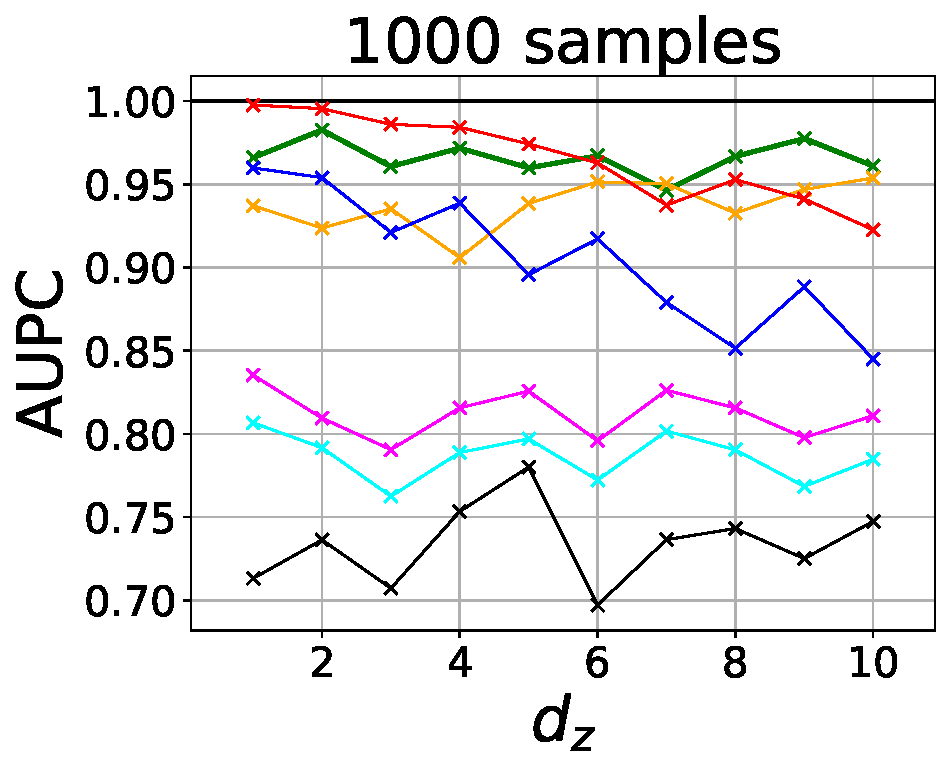
\includegraphics[height=2.3cm]{new_figures_lap/nsamples_fixed_1000_strobl_dim_1_10_aupc.pdf} & 
% 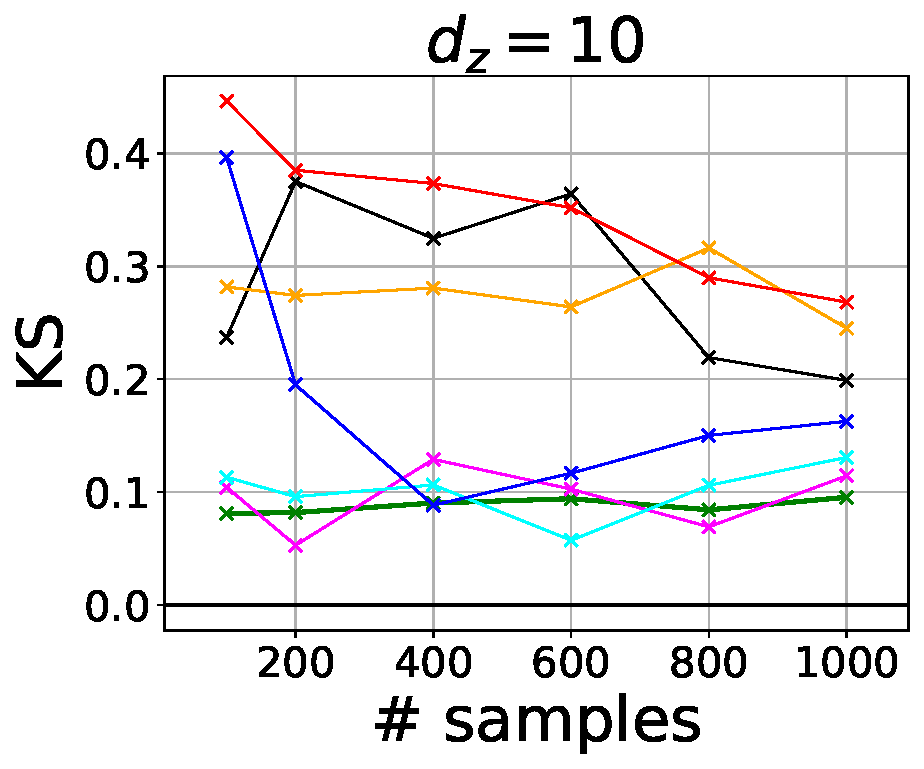
\includegraphics[height=2.3cm]{new_figures_lap/dim_fixed_10_strobl_ks.pdf}& 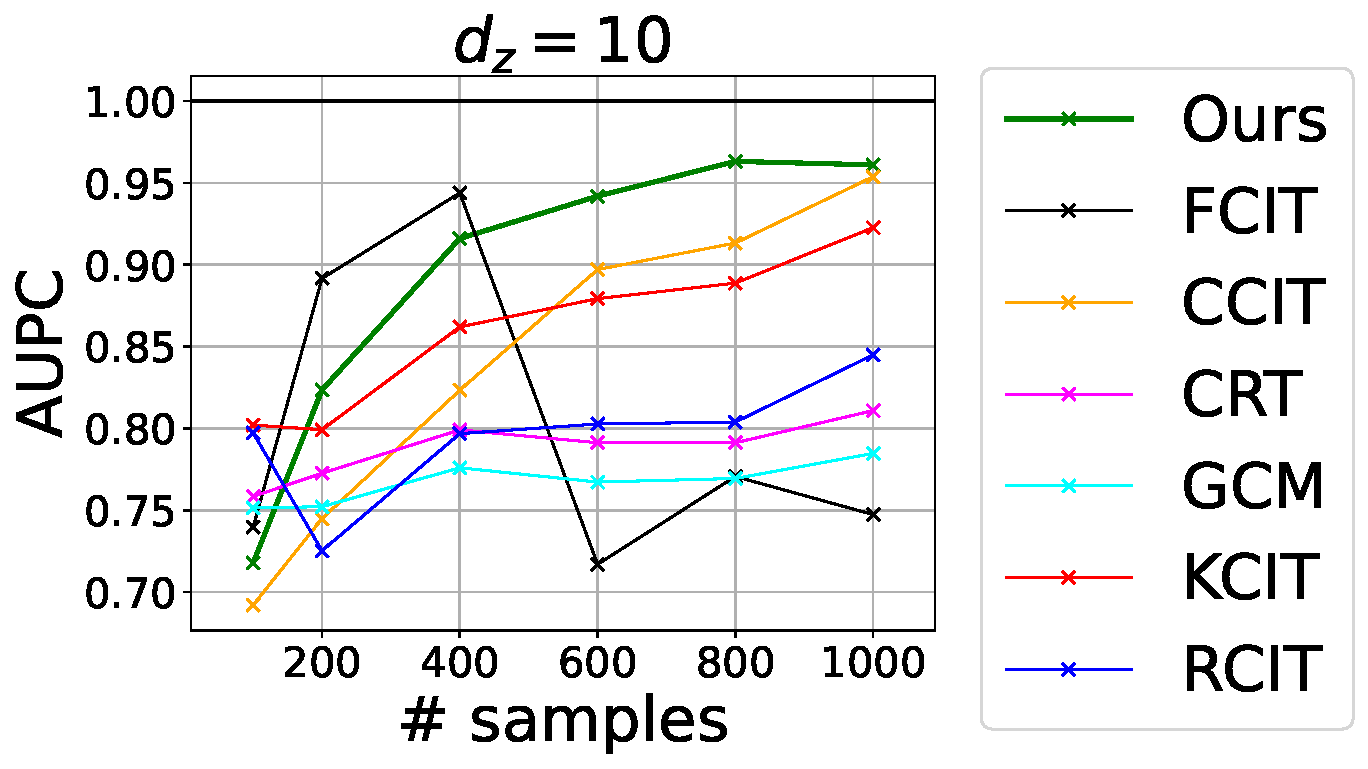
\includegraphics[height=2.3cm]{new_figures_lap/dim_fixed_10_strobl_aupc.pdf} 
% \end{tabular}
% \caption{Comparison of the KS statistic and the AUPC of our testing procedure with other SoTA tests on the two problems presented in Eq.~\eqref{exp-strobl-h0} and Eq.~\eqref{exp-strobl-h1}  with Laplace noises. Each point in the figures is obtained by repeating the experiment for 100 independent trials. (\emph{Left, middle-left}): the KS statistic and AUPC (respectively) obtained by each test when varying the dimension $d_z$ from 1 to 10; here, the number of samples $n$ is fixed and equals to $1000$. (\emph{Middle-right, right}): the KS and AUPC (respectively), obtained by each test when varying the number of samples $n$ from 100 to 1000; here, the dimension $d_z$ is fixed and equals to $10$.
% \label{fig-exp-strobl-ks-laplace}}
% \vspace{-0.3cm}
% \end{figure*}


\begin{figure*}[h]
\begin{tabular}{cccc} 
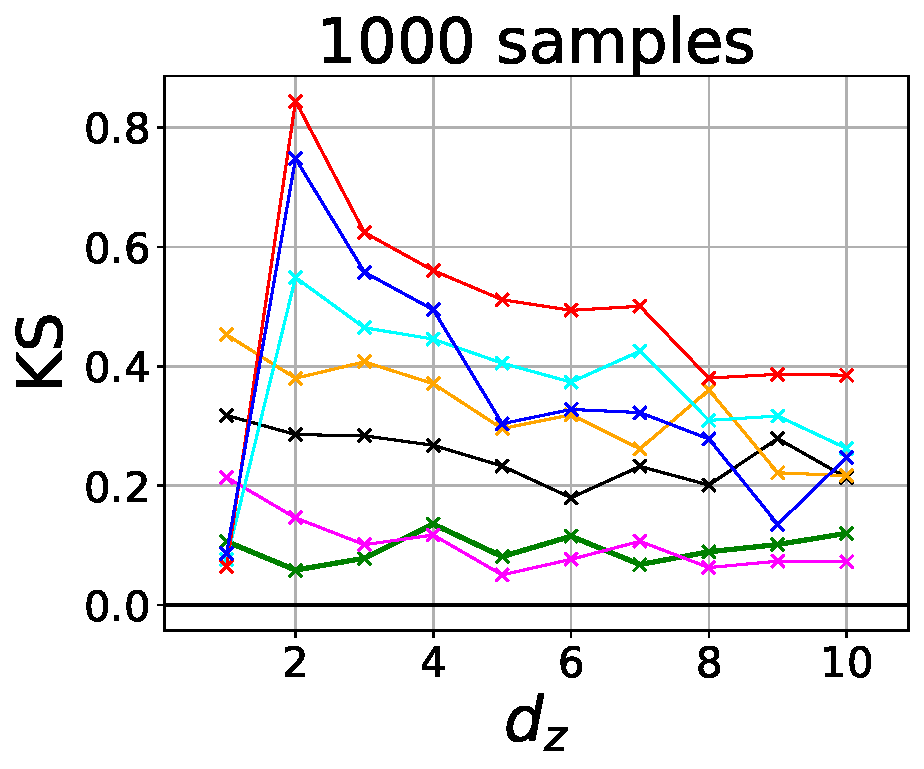
\includegraphics[height=2.3cm]{sections/appendix/independence_testing_kernel/new_figures_lap/nsamples_fixed_1000_li_dim_1_10_ks.pdf}& 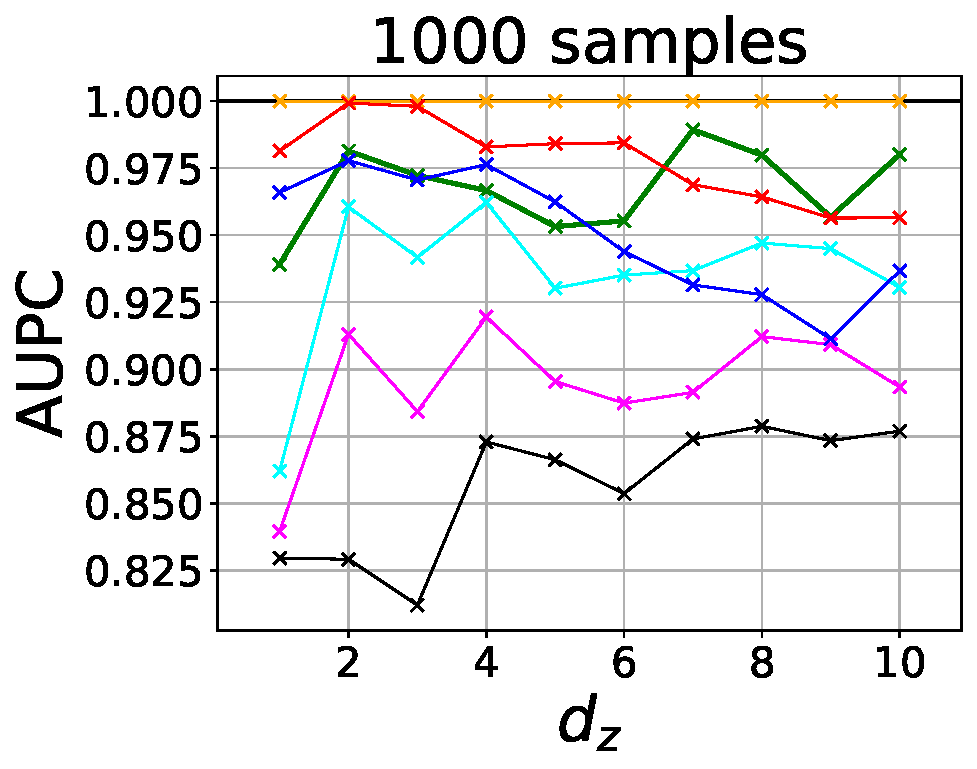
\includegraphics[height=2.3cm]{sections/appendix/independence_testing_kernel/new_figures_lap/nsamples_fixed_1000_li_dim_1_10_aupc.pdf} & 
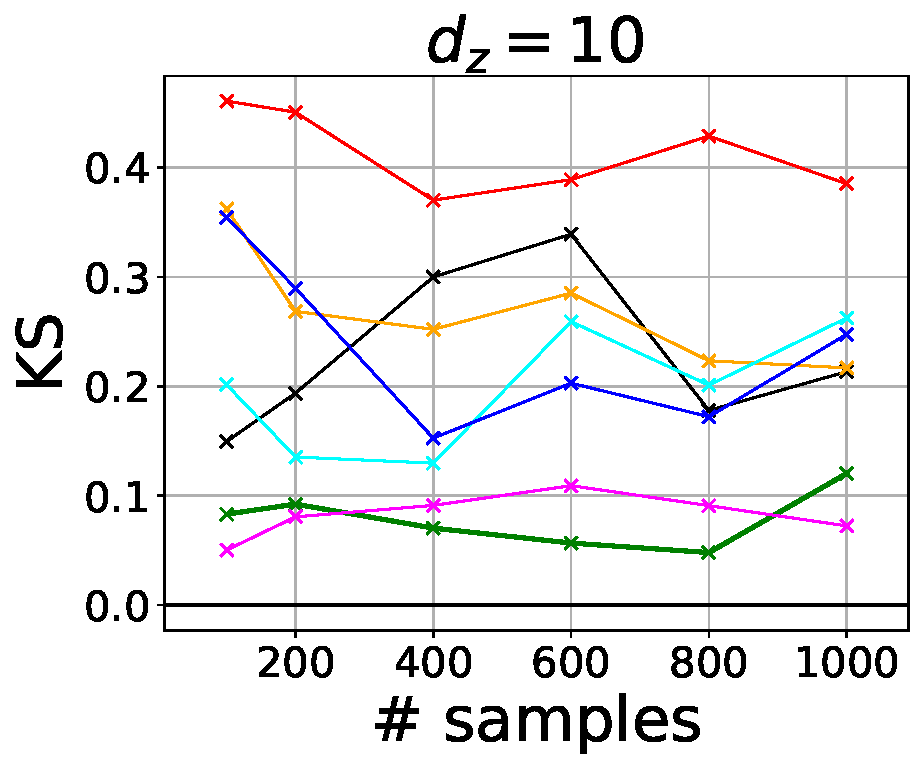
\includegraphics[height=2.3cm]{sections/appendix/independence_testing_kernel/new_figures_lap/dim_fixed_10_li_ks.pdf}& 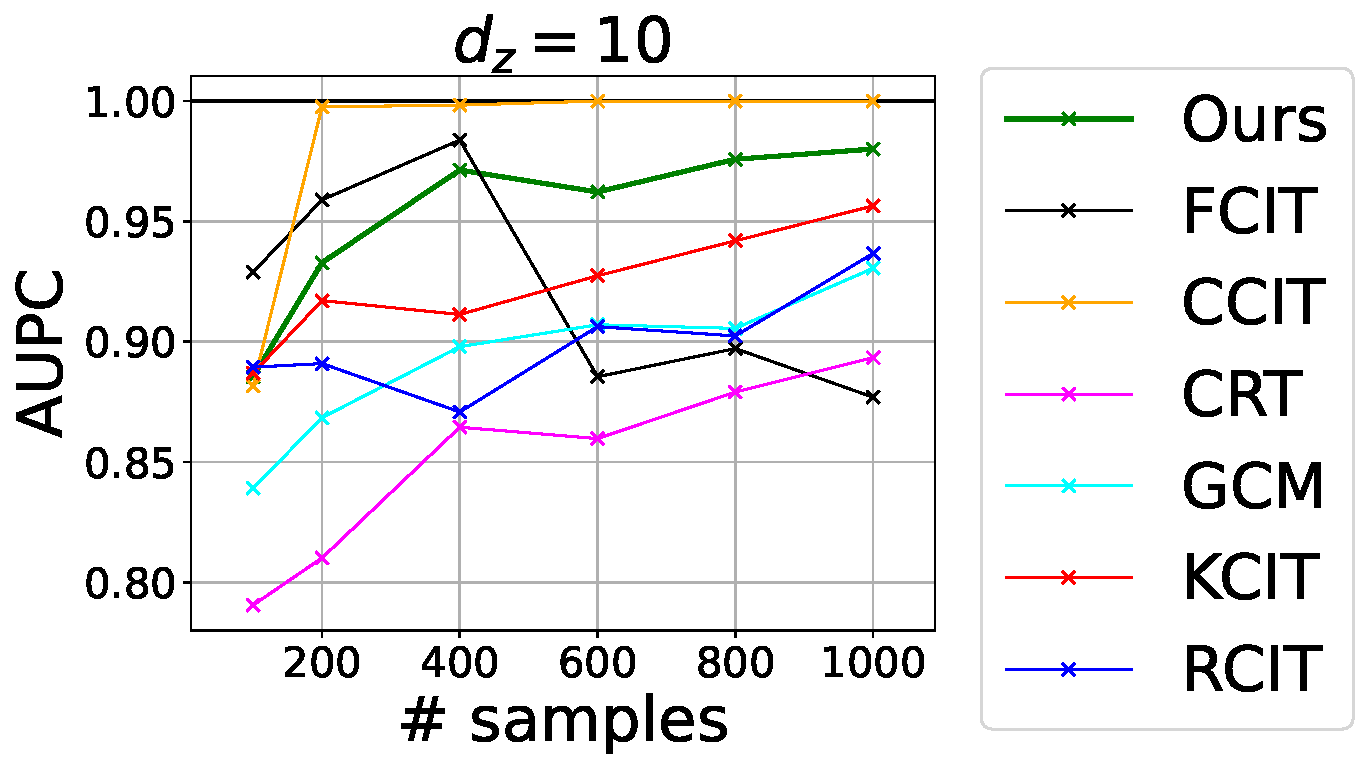
\includegraphics[height=2.3cm]{sections/appendix/independence_testing_kernel/new_figures_lap/dim_fixed_10_li_aupc.pdf} 
\end{tabular}
\caption{Comparison of the KS statistic and the AUPC of our testing procedure with other SoTA tests on the two problems presented in Eq.~\eqref{li-exp-h0} and Eq.~\eqref{li-exp-h1}  with Laplace noises. Each point in the figures is obtained by repeating the experiment for 100 independent trials. (\emph{Left, middle-left}): the KS statistic and AUPC (respectively) obtained by each test when varying the dimension $d_z$ from 1 to 10; here, the number of samples $n$ is fixed and equals to $1000$. (\emph{Middle-right, right}): the KS and AUPC (respectively), obtained by each test when varying the number of samples $n$ from 100 to 1000; here, the dimension $d_z$ is fixed and equals to $10$.
\label{fig-exp-li-ks-laplace}}
\vspace{-0.4cm}
\end{figure*}



\textbf{Effects of $p$, $J$ and $r$.} Our first experiment studies the effects of $p$ and $J$ on our proposed method. In addition we investigate the sensitivity of the method when varying the rank regression $r$ both in term of performance and time. To do so, we follow the synthetic experiment proposed in~\cite{strobl2019approximate}. To evaluate the type-I error, we generate data that follows the model:
\begin{align}
\label{exp-strobl-h0}
    X=f_1(\varepsilon_x), \ Y=f_2(\varepsilon_y),~\text{and Z}\sim\mathcal{N}(0_d,I_{d_z}),
\end{align}
where $Z$, $\varepsilon_x$, and $\varepsilon_y$ are samples from jointly independent standard Gaussian or Laplace distributions, and $f_1$ and $f_2$ are smooth
functions chosen uniformly from the set $\{(\cdot), (\cdot)^2, (\cdot)^3, \tanh(\cdot), \exp(-|\cdot|)\}$. To compare the power of the tests, we also consider the model:
\begin{align}
\label{exp-strobl-h1}
    X=f_1(\varepsilon_x +0.8\varepsilon_b), Y=f_2(\varepsilon_y+0.8\varepsilon_b),
\end{align}
where $\varepsilon_b$ is sampled from a standard Gaussian or Laplace distribution. In Figure~\ref{fig-exp-param}, we compare the KS statistic and the AUPC of our method when varying $p$ and $J$. That figure shows that (i) our method is robust to the choice of $p$, and (ii) the performances of the test do not necessarily increase as $J$ increases. In Figure~\ref{fig-rn-dependence} (see Appendix~\ref{sec-rank-rn}), we also show that the power of the test is not very sensible to the choice of the rank $r$, however, we observe that the type-I error decreases as the rank $r$ increases. Armed with theses observations, in the following experiments, we always set $p=2$, $J=5$ and $r=n$ for our method.


\textbf{Illustrations of our theoretical findings.} 
The following experiment confirms that validity of our theoretical results from Propositions~\ref{prop:oracle-law} and \ref{prop:norm-law}. For that purpose, we generate two synthetic data sets for which either $H_0$ or $H_1$ holds. Concretely, we define a first triplet $(X,Y,Z)$ as follows:
\begin{align}
\label{exp-illustration-h0}
X = \text{P}_1(Z) + \varepsilon_x,~~Y = \text{P}_1(Z) + \varepsilon_y.
\end{align}
Above, $\varepsilon_x$ and $\varepsilon_y$ follow two independent standard normal distributions, $Z\sim \mathcal{N}(0_{d_z},\Sigma)$ with $\Sigma\in\mathbb{R}^{d_z\times d_z}$. The covariance matrix $\Sigma$  is obtained by multiplying product of a random matrix whose entries are independent and follow standard normal distribution, by its transpose, and $\text{P}_1$ is a projection onto the first coordinate. As a result, in this case, we have that $X\perp Y \mid Z$. We also consider a modification of the above data generating function for which $H_1$ holds. This is done by adding a noise component $\varepsilon_b$ that is shared across $X$ and $Y$ as follows:
\begin{align}
\label{exp-illustration-h1}
X = \text{P}_1(Z) + \varepsilon_x + \varepsilon_b,~~ Y = \text{P}_1(Z) + \varepsilon_y + \varepsilon_b,
\end{align}
where $\varepsilon_b$ follows the standard normal distribution. Since we consider \emph{Gaussian kernels}, we can obtain an explicit formulation of $\mathbb{E}_{\ddot{X}}\left[k_{\mathcal{\ddot{X}}}(\mathbf{t}^{(1)}_j,\ddot{X})|Z=\cdot\right]$ and $\mathbb{E}_{Y}\left[k_{\mathcal{Y}}(t^{(2)}_j,Y)|Z=\cdot\right]$ for both data generation functions. See Appendix~\ref{sec-theoritical-findings} for more details. 
Consequently, we are able to compute both the normalized version of our oracle statistic $\widehat{\text{CI}}_{n,p}$ and our approximate normalized statistic $\widetilde{\text{NCI}}_{n,r,p}$. In Figure~\ref{fig-illustation-theory}, we show that both statistics manage to recover the asymptotic distribution under $H_0$, and reject the null hypothesis under $H_1$. In addition, we show that in the high dimensional setting, only our optimized version of $\widetilde{\text{NCI}}_{n,r,p}$---obtained by optimizing the hyperparameters involved in the RLS estimators of our statistic---manages to recover the asymptotic distribution under $H_0$.





\textbf{Comparisons with existing tests.} In our next experiments, we compare the performance of our method (implemented with the optimized version of our statistic) with state-of-the-art techniques for conditional independence testing. We first study the two data generating functions from \eqref{exp-strobl-h0} and \eqref{exp-strobl-h1}. For each of these problems, we consider two settings. In the first, we fix the dimension $d_z$ while varying the number of samples $n$. In the second, we fix the number of samples while varying the dimension of the problem. To evaluate the performance of the tests, we compare the type-I errors at level $\alpha=0.05$ under the first model~\eqref{exp-strobl-h0}, and, for second model~\eqref{exp-strobl-h1}, we evaluate the power of the test by presenting the type-II error. Figures~\ref{fig-exp-strobl-type} (Gaussian case) and \ref{fig-exp-strobl-laplace-supp} (Laplace case) demonstrate that our method consistently controls the type-I error and obtains a power similar to the best SoTA tests. In Figures~\ref{fig-exp-strobl-ks-supp} and \ref{fig-exp-strobl-ks-laplace-supp}, we also compare the KS statistic and the AUPC of the different tests, and obtain similar conclusions. In addition, we investigate the high dimensional regime and show in Figure~\ref{fig-exp-strobl-highdim-gaussian-supp} and \ref{fig-exp-strobl-highdim-laplace-supp} that our test is the only one which manages to control the type-I error while being competitive in term of power with other methods. See Appendix~\ref{sec-exp-storbl} for more details. 


We now conduct another series of experiments that build upon the synthetic data sets presented in~\citep{zhang2012kernel,li2020nonparametric,doran2014permutation,BellotS19}.
To compare type-I error rates, we generate simulated data for which $H_0$ is true:
\begin{align}
\label{li-exp-h0}
X=f_1\left(\bar{Z}+\varepsilon_x\right),Y=f_2\left(\bar{Z}+\varepsilon_y\right).
\end{align}
Above, $\bar{Z}$ is the average of $Z=(Z_1,\cdots,Z_{d_z})$, $\varepsilon_x$ and $\varepsilon_y$ are sampled independently from a standard Gaussian or Laplace distribution, and $f_1$ and $f_2$ are smooth
functions chosen uniformly from the set $\{(\cdot), (\cdot)^2, (\cdot)^3, \tanh(\cdot), \exp(-|\cdot|)\}$. To evaluate the power, we consider the following data generating function:
\begin{align}
\begin{aligned}
\label{li-exp-h1}
 X=f_1\left( \bar{Z}+\varepsilon_x\right)+\varepsilon_b,Y=f_2\left(\bar{Z}+\varepsilon_y\right)+\varepsilon_b,
\end{aligned}
\end{align}
where $\varepsilon_b$ is a standard Gaussian or Laplace distribution. 
% We now conduct another series of experiments that build upon the synthetic data sets presented in~\cite{strobl2019approximate}. To evaluate the type-I error, we generate data that follows the model:
% \begin{align}
% \label{exp-strobl-h0}
%     X=f_1(\varepsilon_x), \ Y=f_2(\varepsilon_y),~\text{and Z}\sim\mathcal{N}(0_d,I_{d_z}),
% \end{align}
% where $Z$,   $\varepsilon_x$, and $\varepsilon_y$ are samples from jointly independent standard Gaussian or Laplace distributions depending on the experiment, and $f_1$ and $f_2$ are smooth
% functions chosen uniformly from the set $\{(\cdot), (\cdot)^2, (\cdot)^3, \tanh(\cdot), \exp(-|\cdot|)\}$. To compare the power of the tests, we also consider the model:
% \begin{align}
% \label{exp-strobl-h1}
%     X=f_1(\varepsilon_x +0.8\varepsilon_b), Y=f_2(\varepsilon_y+0.8\varepsilon_b),
% \end{align}
% where $\varepsilon_b$ is sampled from a standard Gaussian or Laplace distribution depending on the experiment. 
As in the previous experiment, for each model, we study two settings by either fixing the dimension $d_z$, or the sample size $n$. In Figure~\ref{fig-exp-li-ks-laplace} (Laplace case) and~\ref{fig-exp-li-ks-gauss-supp} (Gaussian case), we compare the KS and the AUPC of our method with the SoTA tests and demonstrate that our procedure manages to be powerful while controlling the type-I error. In Figures~\ref{fig-exp-li-type-supp} and \ref{fig-exp-li-laplace-supp}, we also compare the type-I and type-II errors of the different tests, and obtain similar conclusions. In addition, we investigate the high dimensional regime and show in Figure~\ref{fig-exp-li-highdim-gauss-supp} and \ref{fig-exp-li-highdim-laplace-supp} that our test outperforms all the other proposed methods in most of the settings. See Appendix~\ref{sec-exp-li} for more details.



% \paragraph{Real world experiment} Finally we test our procedure on a real world dataset. We reproduced the experiment of~\citep{BellotS19}. We use the subset of the CCLE data~\citep{barretina2012cancer} relating to the drug PLX4720; the dataset is composed 474 cancer cell lines described by 466 genetic mutations. As the ground truth causal links are unknown, effectively evaluating conditional dependence on real data is difficult .









% \subsection{Illustrations of our theoretical findings}
% Here we aim at illustrating our theoretical results obtained in Proposition~\ref{prop:rls-law} to show the distribution of our statistics under the null hypothesis. As in \citep{zhang2012kernel,doran2014permutation,BellotS19}, we generate synthetic data that follows the post non-linear noise model. Concretely, we define the triplet $(X,Y,Z)$ as follows:
% \begin{align*}
%     H_0:~& X = f(A_fZ + \varepsilon_f),\quad Y = g(A_gZ + \varepsilon_g)
% \end{align*}
% where $A_{f}, A_g$ and $A_h$ are vectors that result in univariate $X$ and $Y$. The entries in the three vectors and the parameter $\beta$ are all drawn from the $\text{Uniform}$ distribution on the $[0,1]$ interval. The noise parameters $\varepsilon_f, \varepsilon_g$, and $\varepsilon_h$ are sampled from the normal distribution with a zero mean and variance of $0.025$. The choice of the non-linear functions $f$ and $g$ affect the complexity of the statistical test. We follow \citep{BellotS19} and consider the case where $f=g=tanh$. We draw the entries of $Z$ from $\mathcal{N}(0,1)$. The number of samples considered is $n=1000$ and the dimension of the problems are $d_1=d_2=d_3=1$. As we have access to a closed expression of the density of the $\chi^2(J)$, we consider only the case when $p=2$ and we repeat $1000$ times the experiment in order to obtain the density of our statistics. In Figure~\ref{fig-asymptotic}, we plot the results obtained. We see that our measures converge quickly towards the $\chi^2(J)$ for all $J$, both when applying our RLS-based statistic and its random features relaxation.


% \begin{figure}[!h]
% \begin{center}
% 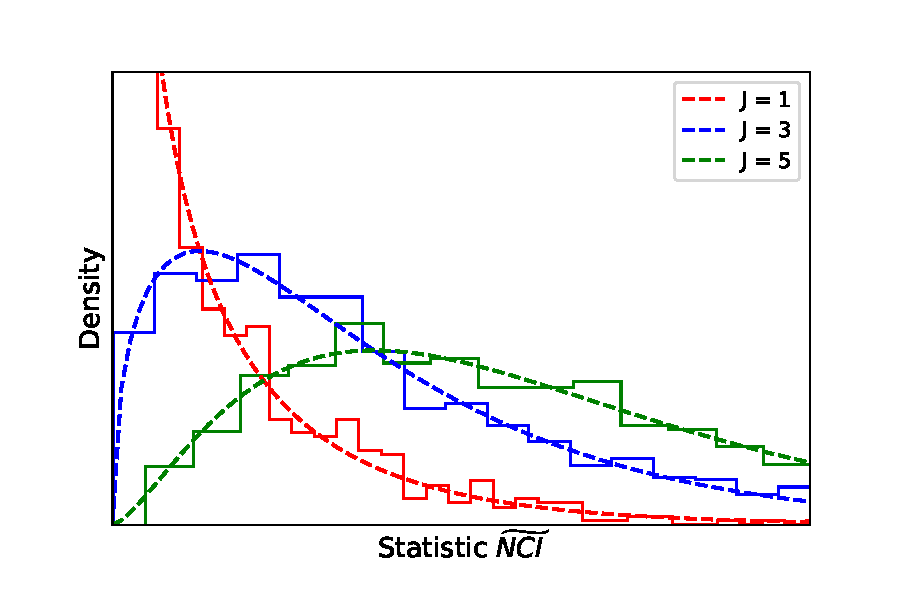
\includegraphics[width=0.45\textwidth]{figures/plot_density_2.pdf}
% 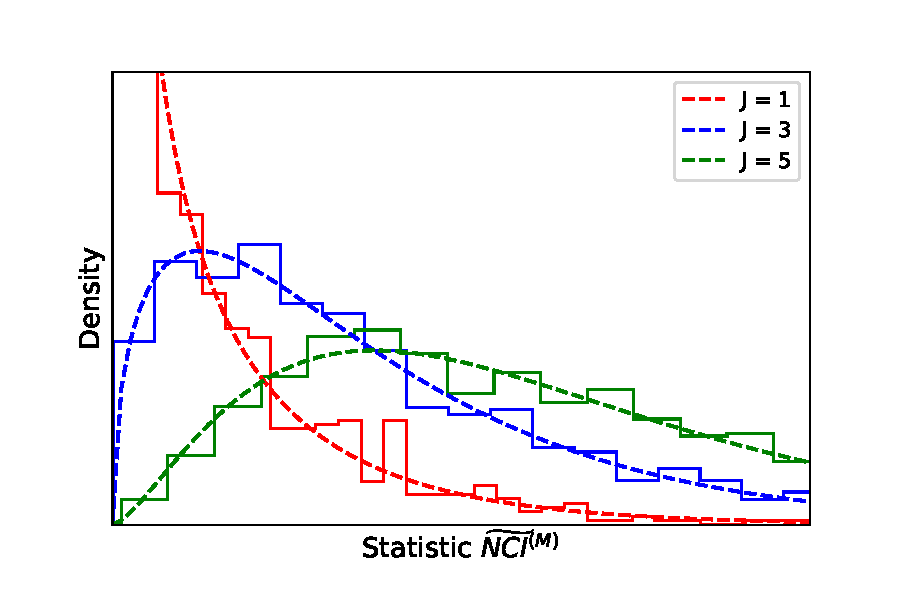
\includegraphics[width=0.45\textwidth]{figures/plot_density_rf_2.pdf}
% \caption{We show the distribution of our statistics for multiple choice of $J$. Here the number of random features is chosen to be $M=100$. Both statistics manage to reach the asymptotic regime of a the $\chi^2(J)$ distribution. \emph{(a)}: Distribution of the regularized least-squares based statistic $\widetilde{\text{NCI}}_{n,r,p}$ under the null hypothesis. \emph{(b)}: Distribution of the random features based statistic $\widetilde{\text{NCI}}^{(M)}_{n,r,p}$ under the null hypothesis. \label{fig-asymptotic}}
% \label{fig:couplings}
% \end{center}
% \vspace{-0.1cm}
% \end{figure}



% as well as the recently proposed conditional randomization test (CRT) \citep{candes2018panning}. The CRT is a powerful approach for conditional independence testing that allows the analyst to deploy any data-driven test statistic $T(\cdot)\in\mathbb{R}$---e.g., a summary statistic that builds upon a complex machine learning model---to examine the dependency structure of $X, Y$, and $Z$. The CRT test repeatedly generates dummy variables $\tilde{X}_i^k, \ 1 \leq i \leq n, \ 1 \leq k \leq K$ from the conditional null and compares the test statistic $T(\{Y_i\}_i,\{\tilde{X}_i\}_i,\{Z_i\}_i)$ to the one evaluated on the original data $T(\{Y_i\}_i,\{{X_i}\}_i,\{Z_i\}_i)$. The sampling from the conditional null is done by generating $\tilde{X}_i \sim P_{X \mid Z}(X \mid Z_i)$, and the p-value of the test is given by
% \begin{equation*}
%     p_{\text{CRT}} = \frac{1 + \sum_{i=1}^K \mathbf{1}\left\{t^* \leq T(\{Y_i\}_i,\{\tilde{X}_i^k\}_i,\{Z_i\}_i) \right\}}{K+1}.
% \end{equation*}
% Above, $t^* = T(\{Y_i\}_i,\{{X}\}_i,\{Z\}_i)$ is the statistic evaluated on the original data points.

% In practice, the conditional distribution $P_{X \mid Z}$---required to generate the dummy variables---is unknown. Following \citep{candes2018panning,BellotS19}, we use the observed data points to approximate the first two moments of this distribution. Importantly, the CRT may generate invalid p-values when provided with a poor approximation of $P_{X \mid Z}$. Indeed, recent methods, such as \citep{BellotS19, tansey2018holdout} attempt to move beyond the Gaussianity assumption and approximate $P_{X \mid Z}$ even for complex data sets.

% The choice of the test statistic affects the power of CRT. In our experiments, we examine several common scoring functions (see, e.g., \citep{BellotS19}), as listed below.
% \begin{itemize}
%     \item \textbf{CRT-Corr}: we set $T(\{Y_i\}_i,\{{X}\}_i,\{Z\}_i)$ to be the absolute value of the Pearson’s correlation coefficient between $\{X_i\}_i$ and $\{Y_i\}_i$.
%     \item \textbf{CRT-RDC}: we also examine the randomized dependence coefficient \citep{lopez2013randomized} as a measure of non-linear dependence between $\{X_i\}_i$ and $\{Y_i\}_i$.
 
%     \item \textbf{CRT-OLS}: this test statistic is obtained by (i) fitting an ordinary least squares model on the data, aiming to predict $\{Y_i\}_i$ from the pair $\{(X_i,Z_i)\}_i$, and (ii) returning the mean squared prediction error.
 
%     \item \textbf{CRT-KRidge}: in contrast to CRT-OLS, here we fit a kernel ridge regression model to the data, and then use the absolute value of the coefficient of determination (often denoted by $R^2$) as a summary statistic.
        
% \end{itemize}

% \subsection{Simulated data I}
% Here to test the the power of our method, we add to the previous setting a post nonlinear model where $H_1$ hold. More precisely we consider
% \begin{align*}
%     H_0:~& X = f(A_fZ + \varepsilon_f),\quad Y = f(A_gZ + \varepsilon_g) \\
%     H_1:~& Y=f(A_hZ + \beta X + \varepsilon_h),
% \end{align*}
% Moreover here $f$ is chosen among the following functions $\{x, x^2, \tanh{x}\}$. 

% % We compare our methods to KCIT, RCIT, CCIT, and GCIT.\footnote{We implemented KCIT and RCIT using the R package available at \url{https://github.com/ericstrobl/RCIT}. The software package of CCIT is from \url{https://github.com/rajatsen91/CCIT/blob/master/CCIT} and the one of GCIT is available at \url{https://github.com/alexisbellot/GCIT}. For all methods, we use the default set of hyper-parameters.} 


% In all experiments, we fix the number of samples $n$ to $600$ and increase the dimension of $Z$. Figure~\ref{fig:auc1}  compares the type-I error when testing $H_0$ at level $\alpha=0.05$ over 100 independent trials. As can be seen, all methods tend to control the type-I error, including our proposed tests. In Figure~\ref{fig:auc1} we compare the statistical power (higher is better) as a function of the dimension of $Z$. Observe how all the methods perform comparably well for in lower dimensions and depart as the dimensions increases. 

% \subsection{Simulated data II [This is the new data]}

% Following \citep{zhang2012kernel,doran2014permutation,BellotS19}, we generate synthetic data that follows the post non-linear noise model. Concretely, we define the triplet $(X,Y,Z)$ as follows:
% \begin{align*}
%     H_0:~& X = f(A_X Z + \varepsilon_x),\quad Y = f(A_Y Z + \varepsilon_y) \\
%     H_1:~& Y=f(A_Z Z + \beta X + \varepsilon_z),
% \end{align*}
% where $A_{X}, A_Y$ and $A_Z$ are vectors that result in univariate $X$ and $Y$, whose entries are drawn from the $\text{Uniform}(0,1)$ distribution. We set the dimension of $X$ to one and sample the parameter $\beta \in [0,1]$ from the uniform distribution as well. The noise parameters $\varepsilon_x, \varepsilon_y$, and $\varepsilon_z$ are sampled from a normal distribution with zero mean and variance that equals to $0.025$. 




% \begin{table}[]
% \centering
% \begin{tabular}{@{}ccc@{}}
% \toprule
% Setting & Distribution of $Z$                                                                        & Choice of $f$        \\ \midrule
% $H_0$: A  & \multirow{2}{*}{\begin{tabular}[c]{@{}c@{}}Gaussian\\ (mean 0, variance 1)\end{tabular}} & Identity: $f(x) = x$ \\
% $H_0$: B  &                                                                                          & Square: $f(x) = x^2$ \\ \midrule
% $H_0$: C  & \begin{tabular}[c]{@{}c@{}}Laplace\\ (location 0, scale 1)\end{tabular}                  & Identity: $f(x) = x$ \\ \bottomrule
% \end{tabular}
% \caption{Data generating mechanism under $H_0$.} \label{tab:data_H0}
% \end{table}

% The choice of the function $f$, the sampling distribution of the data, and the dimensions of the problem affect the complexity of test. In all experiments, we fix the number of samples $n$ to 600 and increase the dimension of $Z$ from 2 to 250. Table~\ref{tab:data_H0} summarizes three different settings that we examine when $H_0$ is true. 

% Figure ??? compares the type-I error of each method as a function of the dimension of $Z$. Here, we test the null hypothesis $H_0$ at level $\alpha=0.05$ by applying each test to 100 independent data sets. As can be seen, the tests we study tend to control the type-I error only when the dimension of 
% $Z$ is low, except the CRT that works well when the data follows the Gaussian distribution for which $f$ is the identity function. This is expected as we assume $X \mid Z$ to be Gaussian. When $Z$ follows the Laplace distribution, or when $f$ is the square function, the approximation we provide for the conditional distribution is poor, which, in turn, results in a violation of type-I error control. {\color{red} need to see the graphs}

% Next, we examine the power of the tests by generating data for which $H_1$ is true. We follow the same setting as described in Table~\ref{tab:data_H0}, except that now we also sampled $X$ from the same distribution of $Z$. In Figure ??? we plot the power of each test as a function of the dimension of $Z$. Observe how the ?????




% We compare our methods to KCIT, RCIT, CCIT, and GCIT.\footnote{We implemented KCIT and RCIT using the R package available at \url{https://github.com/ericstrobl/RCIT}. The software package of CCIT is from \url{https://github.com/rajatsen91/CCIT/blob/master/CCIT} and the one of GCIT is available at \url{https://github.com/alexisbellot/GCIT}. For all methods, we use the default set of hyper-parameters.} 


%  In Figure ??? we compare the statistical power (higher is better) as a function of the dimension of $Z$. Observe how all the methods perform comparably well for in lower dimensions and depart as the dimensions increases. ADD DETAILS WHEN GRAPHS WILL EXIST :)
    

% \subsection{Simulated data III}

% Herein, we generate synthetic data according to the following model:
% $$Y = f(X^{\top}\beta + \varepsilon ),$$
% where $X\in\mathbb{R}^{d}$ and the noise $\varepsilon \in\mathbb{R}$ is sampled independently from $\mathcal{N}(0,0.05)$. Above, the vector $X$ is generated by (i) independently sampling its entries from the standard Gaussian distribution, and (ii) applying the non-linear cosine function on each entry. We create the vector $\beta \in\mathbb{R}^{d}$ by assigning a non-zero value only in odd locations, where the magnitude of the $j$th non-zero is $1/j$. For example, for $d=7$ we have $\beta = [1, 0, 1/2, 0, 1/3, 0, 1/4]$. Under this construction, every odd coordinate $X_k \in \mathbb{R}$ is independent of $Y$ given $X_{-k} \in  \mathbb{R}^{d-1}$, where the latter is a vector that contains all the elements but the $k$th one. Analogously, every even coordinate $X_j$ is dependent of $Y$ given $X_{-j}$; here, as the index $j$ increases, the dependence is smaller and thus it is more challenging to detect that this variable departs from the null.




% \section{Discussions and conclusion}

% Our results on asymptotic distribution requires more assumptions than the results proposed by~\cite{zhang2012kernel}. Indeed, we need conditions to ensure the convergence rate of the RLS estimator. However, in~\citep{zhang2012kernel}, the proof of their asymptotic law requires assumptions to ours to hold. In~\citep{strobl1702approximate}, to prove their asymptotic distribution, the authors assume to have access to samples from the conditional mean, which is in practice impossible. In our work, by adding Assumptions~\ref{ass:spectrum}-\ref{ass:source}, we show we pr

% \begin{figure}
%     \centering
%     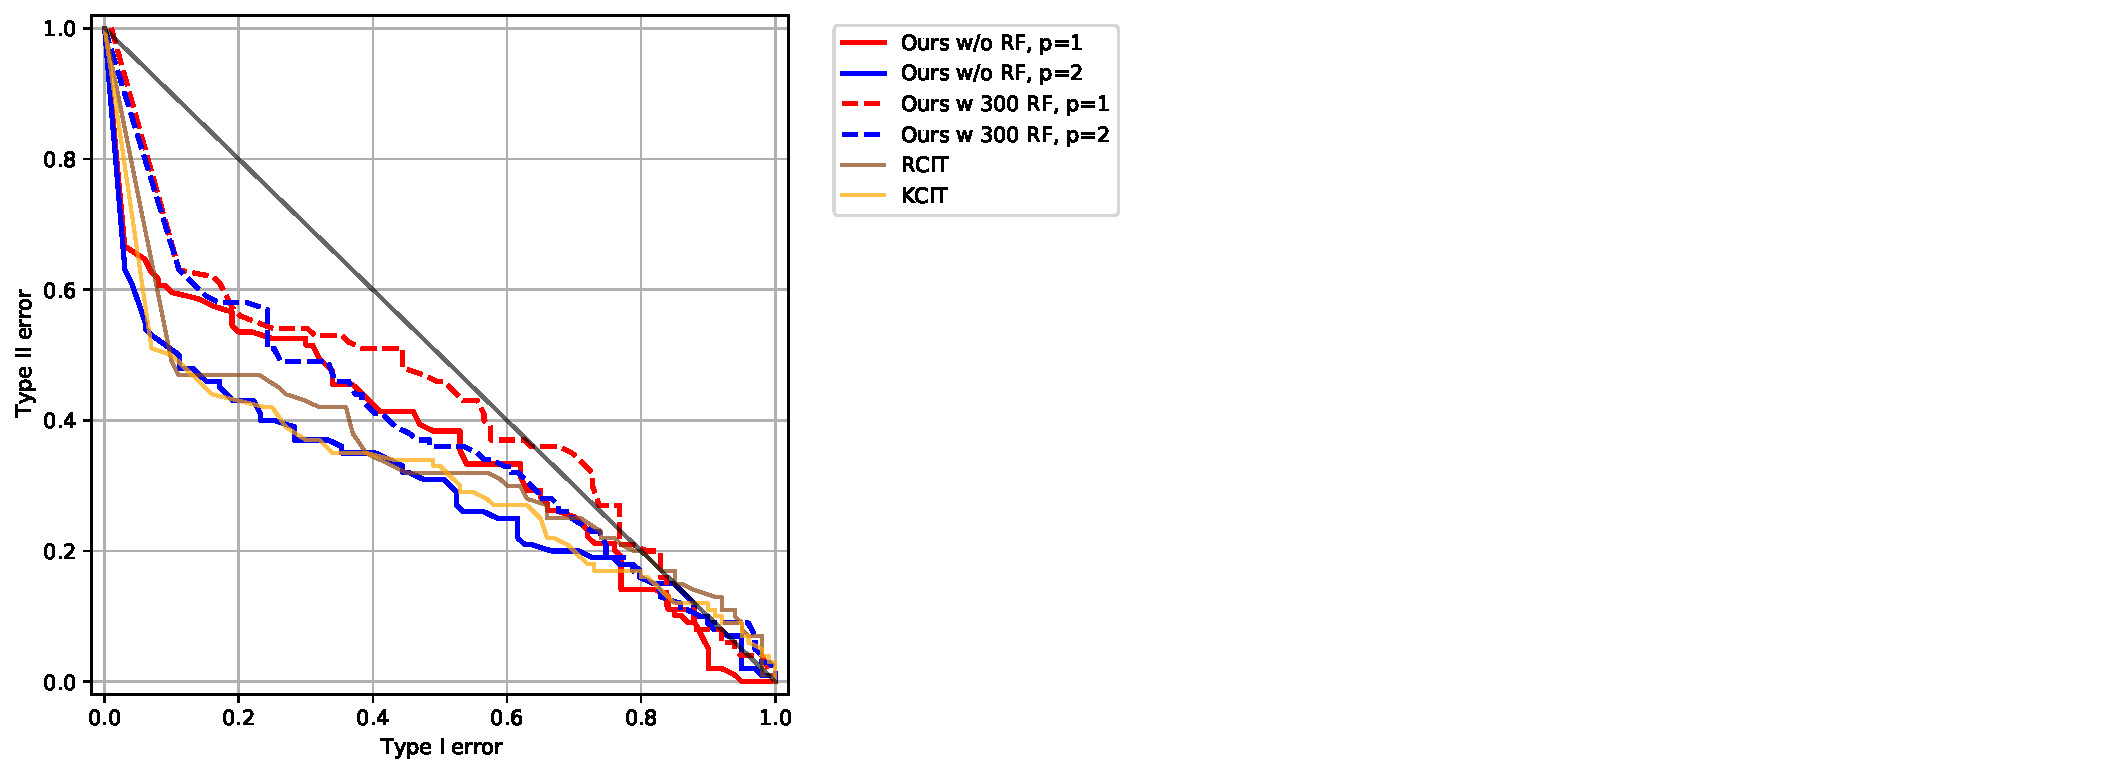
\includegraphics[width=0.85\textwidth]{figures/plots_v1_auc_5_True_square.pdf}
%     \caption{Area under curve comparing our approaches (Section~\ref{sec:42}) with KCIT and RCIT on a $5$ dimensional problem, with $f(x)=x^2$. The number of samples is fixed at $600$, and the results are averaged over $100$ runs. We chose $J=3$ and we optimized the positions of the $t_j$ and the parameters of the gaussian kernels. We fixed the rank of the RLS estimation to $r=300$.}
%     \label{fig:auc1}
% \end{figure}
% \begin{figure}
%     \centering
%     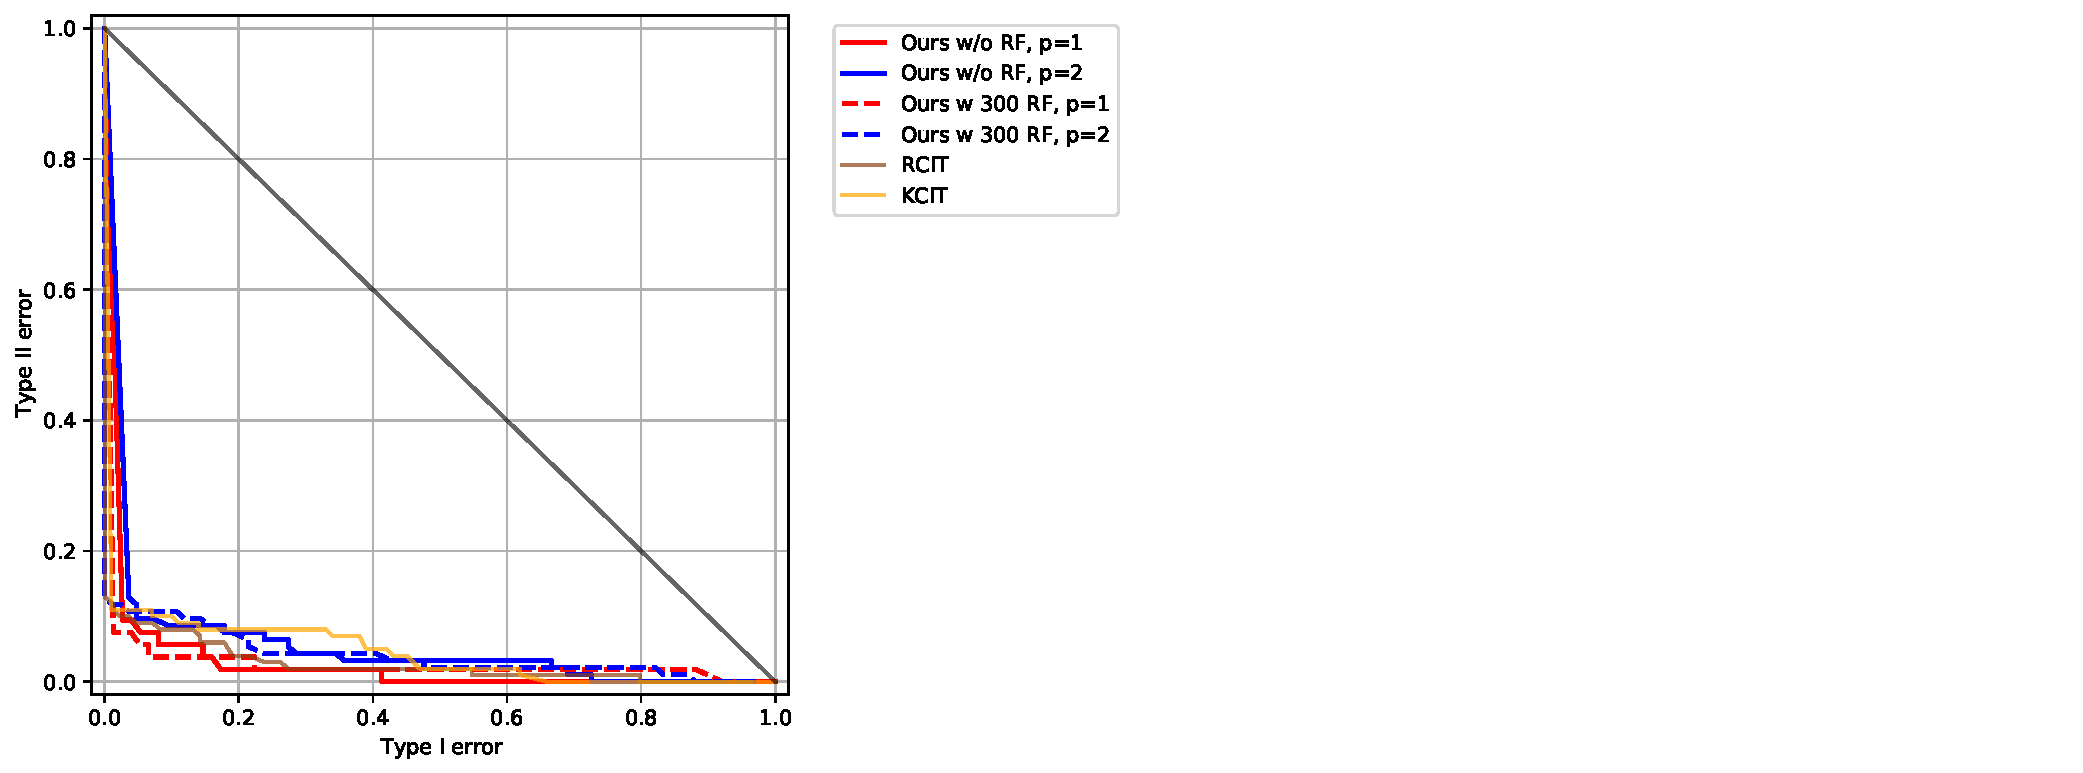
\includegraphics[width=0.85\textwidth]{figures/plots_v2_auc_2_False_gaussian_square.pdf}
%     \caption{Area under curve comparing our approaches (Section~\ref{sec:43}) with KCIT and RCIT on a $2$ dimensional problem, with $f(x)=x^2$. The number of samples is fixed at $600$, and the results are averaged over $100$ runs. We chose $J=3$, we did not optimize the positions of the $t_j$, neither the parameters of the gaussian kernels. We fixed the rank of the RLS estimation to $r=300$.}
%     \label{fig:auc2}
% \end{figure}


% \begin{figure*}
%     \centering
%     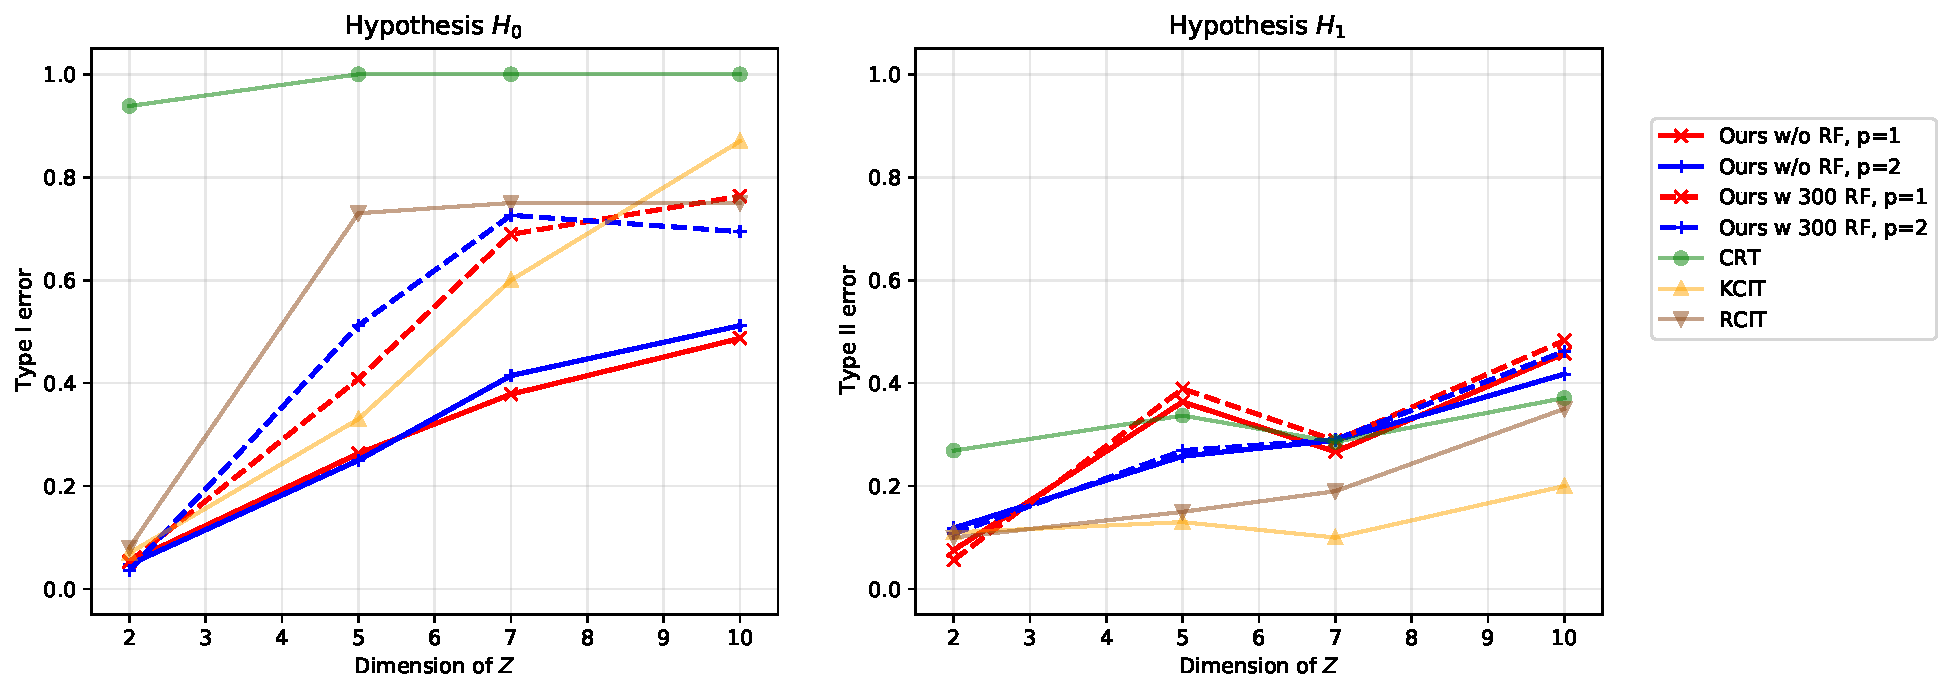
\includegraphics[width=0.9\textwidth]{figures/plots_v2_False_gaussian_square.pdf}
%     \caption{Comparison of our approach with RCIT, KCIT and CRT for various dimension of $Z$. On left, the problem is simulated from $H_0$ and we plotted the Type I error. On right from $H_1$ and we plotted the Type II error. The number of samples is fixed at $600$, and the results are averaged over $100$ runs. We chose $J=3$ , we did not optimize the positions of the $t_j$, neither the parameters of the gaussian kernels. We fixed the rank of the RLS estimation to $r=300$.}
%     \label{fig:type_error}
% \end{figure*}